\documentclass[conference]{IEEEtran}
\IEEEoverridecommandlockouts

\usepackage{cite}
\usepackage{subfigure}
\usepackage{amsmath,amssymb,amsfonts}
\usepackage{algorithmic}
\usepackage{graphicx}
\usepackage{textcomp}
\usepackage{xcolor}
\usepackage{textcomp}
\usepackage{float}
\usepackage{array}
\usepackage{siunitx}
\usepackage{tabularx}
\usepackage{listings}
\usepackage[colorlinks=false]{hyperref}
\def\BibTeX{{\rm B\kern-.05em{\sc i\kern-.025em b}\kern-.08em
    T\kern-.1667em\lower.7ex\hbox{E}\kern-.125emX}}

\setlength{\parindent}{0pt}

% Define the custom column type Y
\newcolumntype{Y}{>{\centering\arraybackslash} m{1.9cm}}

% Define Python colors
\definecolor{codeblue}{rgb}{0.2,0.2,0.6}
\definecolor{codegreen}{rgb}{0.133,0.545,0.133}
\definecolor{codegray}{rgb}{0.5,0.5,0.5}
\definecolor{codepurple}{rgb}{0.58,0,0.82}
\definecolor{backcolour}{rgb}{0.95,0.95,0.92}
% Define Python style
\lstdefinestyle{mystyle}{
    backgroundcolor=\color{backcolour},
    commentstyle=\color{codegreen},
    keywordstyle=\color{codeblue},
    numberstyle=\tiny\color{codegray},
    stringstyle=\color{codepurple},
    basicstyle=\ttfamily\tiny,
    breakatwhitespace=false,
    breaklines=true,
    captionpos=b,
    keepspaces=true,
    numbers=none,
    numbersep=5pt,
    showspaces=false,
    showstringspaces=false,
    showtabs=false,
    tabsize=2
}
% Apply the style to listings
\lstset{style=mystyle}

% Define Arduino colors
\definecolor{arduinoorange}{RGB}{242, 123, 56}
\definecolor{arduinogray}{RGB}{100, 100, 100}
\definecolor{lightgray}{RGB}{240, 240, 240}
% Define Arduino style
\lstdefinestyle{Arduino}{
  language=C++,
  basicstyle=\tiny\ttfamily,
  backgroundcolor=\color{lightgray},
  keywordstyle=\color{arduinoorange},
  commentstyle=\color{arduinogray},
  stringstyle=\color{blue},
  tabsize=2,
  showspaces=false,
  showstringspaces=false
}
% Apply the style to listings
\lstset{style=Arduino}

% Redefine \texttt to make the font smaller
\let\oldtexttt\texttt
\renewcommand{\texttt}[1]{\small\oldtexttt{#1}}

\title{Robotics and Mechatronics\\
{\LARGE Mini Project Four}
}

\author{
    \IEEEauthorblockN{Abolfazl Nateghi}
    \IEEEauthorblockA{\small \textit{School of Mechanical Engineering} \\
    \footnotesize \textit{College of Engineering, University of Tehran \,}\\
    % Tehran, Iran \\
    abolfazlnateghi@ut.ac.ir \\
    SID: 810699275}
    \and
    \IEEEauthorblockN{Hamed Moshtaghian}
    \IEEEauthorblockA{\small \textit{School of Mechanical Engineering} \\
    \footnotesize \textit{College of Engineering, University of Tehran \,}\\
    % Tehran, Iran \\
    hamedmoshtaghian@ut.ac.ir \\
    SID: 810699265}
    \and
    \IEEEauthorblockN{Mohammad Montazeri}
    \IEEEauthorblockA{\small \textit{School of Mechanical Engineering} \\
    \footnotesize \textit{College of Engineering, University of Tehran \,}\\
    % Tehran, Iran \\
    mohammadmontazeri@ut.ac.ir \\
    SID: 810699269}
}


\begin{document}

\maketitle

\begin{abstract}
  This project integrates YOLO for object detection and FastSAM for object segmentation, creating a robust real-time visual analysis system. Combining YOLO's speed and accuracy with FastSAM's segmentation precision enhances performance, accuracy, and efficiency in visual tasks.
\end{abstract}

\begin{IEEEkeywords}
  YOLO, FastSAM, object, detection, segmentation, boundary box, dataset
\end{IEEEkeywords}

\section{Introduction}
Object detection and segmentation are essential in computer vision applications like autonomous driving and surveillance. YOLO excels in real-time object detection but lacks detailed segmentation capabilities. FastSAM provides precise segmentation, making it an ideal complement to YOLO. This project combines YOLO's detection with FastSAM's segmentation to create a system that enhances accuracy and efficiency in real-time visual analysis.
\vspace{8px}

\section{Problem 1: YOLO different versions}
YOLO (You Only Look Once) is a popular object detection algorithm that has evolved through multiple versions. Each version has introduced significant changes and improvements over the previous ones. Here is a brief overview of some key differences introduced in each version:

\subsection*{YOLOv1 to YOLOv2 (YOLO9000)}
Difference: Improved Bounding Box Prediction
\begin{itemize}
  \item YOLOv1: Used fully connected layers to predict bounding box coordinates, which was less accurate.
  \item YOLOv2: Introduced the use of anchor boxes to predict bounding boxes. This made the model more accurate and capable of handling objects of varying sizes more effectively. YOLOv2 also utilized batch normalization and higher resolution input images (416x416) for better detection accuracy.
\end{itemize}

\subsection*{YOLOv2 to YOLOv3}
Difference: Multi-Scale Predictions and Feature Pyramid Network (FPN)
\begin{itemize}
  \item YOLOv2: Predicted bounding boxes at a single scale.
  \item YOLOv3: Added multi-scale predictions by using feature maps at three different scales (large, medium, small). This allowed YOLOv3 to detect objects more effectively at different sizes and improved the detection of small objects significantly. Additionally, YOLOv3 incorporated a Feature Pyramid Network (FPN), enabling the model to process features from different scales within the image, leading to better detection of both small and large objects.
\end{itemize}

\subsection*{YOLOv3 to YOLOv4}
Difference: Bag of Freebies, Bag of Specials, and Authorship Shift
\begin{itemize}
  \item YOLOv3: Utilized a straightforward architecture without many of the enhancements seen in modern object detectors.
  \item YOLOv4: Introduced various techniques collectively termed as "Bag of Freebies" (e.g., data augmentation, class label smoothing) and "Bag of Specials" (e.g., Mish activation, Cross Stage Partial connections). These enhancements improved the training process and overall performance without significantly increasing the inference cost. Additionally, YOLOv4 focused on making the model lighter and faster by utilizing techniques like Spatial Pyramid Pooling (SPP) to extract features efficiently and achieve faster inference times. This version also saw a shift in authorship, with the community and new developers continuing the work on the model.
\end{itemize}

\subsection*{YOLOv4 to YOLOv5}
Difference: Optimized Framework and Codebase
\begin{itemize}
  \item YOLOv4: Mainly focused on algorithmic improvements and was implemented in the Darknet framework.
  \item YOLOv5: Not officially released by the original authors but became popular through its PyTorch implementation. YOLOv5 offered an optimized codebase that was easier to use, faster to train, and more accessible to a broader audience due to its integration with PyTorch, leading to widespread adoption and improvements in ease of deployment and community contributions.
\end{itemize}

\subsection*{YOLOv5 to YOLOv6}
Difference: Decoupled Head
\begin{itemize}
  \item YOLOv5: Continued to use a coupled head for classification and regression tasks.
  \item YOLOv6: Introduced a decoupled head for classification and regression, which allows these tasks to be handled more independently, improving accuracy and inference speed by optimizing the architecture for each task separately.
\end{itemize}

\subsection*{YOLOv6 to YOLOv7}
Difference: Reparameterized Convolutions and Model Efficiency
\begin{itemize}
  \item YOLOv6: Focused on structural improvements but did not employ reparameterization techniques.
  \item YOLOv7: Utilized reparameterized convolutions and made further optimizations in the architecture to improve the model's efficiency and accuracy, making YOLOv7 the state-of-the-art in terms of speed and accuracy trade-offs at the time of its release.
\end{itemize}

\subsection*{YOLOv7 to YOLOv8}
Difference: Advanced Training Techniques, Enhanced Features, and Authorship Shift
\begin{itemize}
  \item YOLOv7: Incorporated reparameterized convolutions and focused on efficiency.
  \item YOLOv8: Further improved training techniques, introduced new data augmentation strategies, and made enhancements in feature pyramid networks, boosting both the training efficiency and detection performance across various object detection benchmarks. Additionally, YOLOv8 boasts improved accuracy for small objects by utilizing an EfficientNet backbone network, known for good performance with limited resources, leading to better detection of smaller objects in the image.
\end{itemize}

\section{Problem 2: mAP score}
\subsection*{Step-by-Step Calculation of mAP}

\begin{enumerate}
  \item \textbf{Detection and Ground Truth:}
        \begin{itemize}
          \item \textbf{Detection:} The model generates a set of bounding boxes and associated confidence scores for objects in an image.
          \item \textbf{Ground Truth:} The actual locations and classes of objects in the image.
        \end{itemize}

  \item \textbf{Sorting by Confidence Score:}
        \begin{itemize}
          \item The detected bounding boxes are sorted in descending order based on their confidence scores.
        \end{itemize}

  \item \textbf{Intersection over Union (IoU) Calculation:}
        \begin{itemize}
          \item For each detected bounding box, the Intersection over Union (IoU) with each ground truth box is calculated. IoU is defined as the area of overlap between the predicted bounding box and the ground truth box divided by the area of their union.
        \end{itemize}

  \item \textbf{Assigning Detections:}
        \begin{itemize}
          \item A detected bounding box is considered a True Positive (TP) if its IoU with a ground truth box exceeds a certain threshold (commonly 0.5).
          \item It is marked as a False Positive (FP) if it does not match any ground truth box or if the IoU is below the threshold.
          \item Ground truth boxes that are not matched with any detection are counted as False Negatives (FN).
        \end{itemize}

  \item \textbf{Precision and Recall Calculation:}
        \begin{itemize}
          \item \textbf{Precision} is the ratio of true positives to the sum of true positives and false positives:
                \[
                  \text{Precision} = \frac{TP}{TP + FP}
                \]
          \item \textbf{Recall} is the ratio of true positives to the sum of true positives and false negatives:
                \[
                  \text{Recall} = \frac{TP}{TP + FN}
                \]
        \end{itemize}

  \item \textbf{Precision-Recall Curve:}
        \begin{itemize}
          \item Precision and recall are calculated at various thresholds, and a precision-recall curve is plotted.
        \end{itemize}

  \item \textbf{Average Precision (AP):}
        \begin{itemize}
          \item Average Precision (AP) is the area under the precision-recall curve. It summarizes the shape of the precision-recall curve into a single value by computing the integral of the precision with respect to recall.
          \item To calculate AP, precision is usually interpolated to ensure that the precision value does not decrease with increasing recall. One common interpolation method is to use the maximum precision for all recall levels greater than the current recall:
                \[
                  p_{\text{interp}}(r) = \max_{r' \geq r} p(r')
                \]
          \item AP is then computed as:
                \[
                  AP = \sum_n [R(n) - R(n-1)] P_{\text{interp}} (R(n))
                \]
                where \(R(n)\) and \(P_{\text{interp}}(R(n))\) are the recall and interpolated precision at the \(n\)-th threshold.
        \end{itemize}

  \item \textbf{Mean Average Precision (mAP):}
        \begin{itemize}
          \item mAP is the mean of the AP values for all object classes. If there are N classes, the
                mAP is:
                \[
                  mAP = \frac{1}{N} \sum_{i=1}^{N} AP_i
                \]
          \item This involves calculating the AP for each class and then averaging these values.
        \end{itemize}
\end{enumerate}

\subsection*{Practical Example}
For instance, suppose you have an object detection task with 3 classes (cat, dog, and car). You would:
\begin{enumerate}
  \item Calculate the AP for each class based on the precision-recall curve for that class.
  \item Average these AP values to get the mAP:
        \[
          mAP = \frac{1}{3} \left(AP_{\text{cat}} + AP_{\text{dog}} + AP_{\text{car}}\right)
        \]
\end{enumerate}

\section{Problem 3: Project dataset}
\subsection{Class Distribution and Health Check}
The dataset provided for this project is examined through \textit{RoboFlow} analysis options (Figure~\ref{fig:prob3-c}). This dataset contains a varying number of images and instances per class:
\begin{table}[H]
  % \caption{}
  \def\arraystretch{1.25}
  \begin{center}
    \begin{tabular}{|ll|ll|ll|}
      \hline
      object           & inst & object           & inst & object         & inst \\
      \hline
      Logo             & 551  & Cup (standing)   & 384  & Tea            & 343  \\
      Cup (laying)     & 337  & Fork             & 314  & Biscuit        & 304  \\
      Knife            & 289  & Spoon            & 282  & Juice (laying) & 240  \\
      Nescafe          & 240  & Tangerine        & 222  & Straw          & 221  \\
      Banana           & 201  & Cake             & 191  & Rani (laying)  & 146  \\
      Nescafe (square) & 144  & Juice (standing) & 138  & Pack           & 114  \\
      Rani (standing)  & 71   &                  &      &                &      \\
      \hline
    \end{tabular}
  \end{center}
\end{table}


The class distribution is uneven, with some classes like ``Logo'' and ``Cup (standing)'' having significantly more instances than underrepresented classes such as ``rani (standing)'' and ``Pack''.

\textbf{Underrepresented Classes}: In the context of machine learning datasets, \textit{underrepresented} refers to classes that have significantly fewer instances compared to other classes in the dataset. This imbalance can affect the model's ability to learn and generalize well, often leading to biased predictions. \\
•	Rani (standing): 71 instances \\
•	Pack: 114 instances \\
•	Juice (standing): 138 instances \\
•	Nescafe (square): 144 instances \\
•	Rani (laying): 146 instances \\

These classes have noticeably fewer instances than the more populated classes such as ``Logo'' with 551 instances. Addressing this imbalance is important for creating a robust and fair model.

\begin{figure}[htbp]
  \centering
  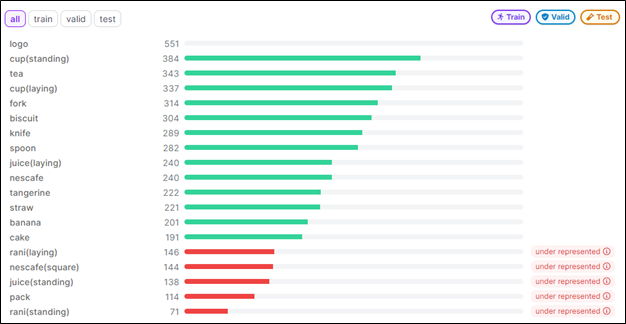
\includegraphics[width=0.49\textwidth]{figures/prob3-a.png}
  \caption{Class distribution of dataset managed in \textit{RoboFlow}}
  \label{fig:prob3-a}
\end{figure}

\subsection{Data Augmentation Necessity}
Data augmentation is crucial in dataset development for several reasons:
\begin{enumerate}
  \item \textbf{Increase Data Volume:} Augmentation techniques create new training examples from existing data by applying transformations such as rotation, translation, and noise addition. This effectively increases the size of the dataset without needing additional data collection.
  \item \textbf{Enhance Model Robustness:} By exposing the model to various altered versions of the original data, it learns to generalize better and becomes more robust to variations in real-world scenarios. This helps in reducing overfitting, as the model does not memorize specific features of the training set but learns to recognize patterns in diverse conditions.
  \item \textbf{Simulate Real-World Variations:} Augmentation helps simulate real-world conditions such as different lighting, angles, and occlusions. This is particularly important for applications involving object detection and recognition in dynamic environments, ensuring that the model performs well under varied conditions.
  \item \textbf{Improve Model Performance:} Diverse training data ensures that the model can handle edge cases and unexpected variations, leading to improved performance metrics such as accuracy, precision, recall, and mean Average Precision (mAP).
\end{enumerate}

\begin{figure}[htbp]
  \centering
  \subfigure{
    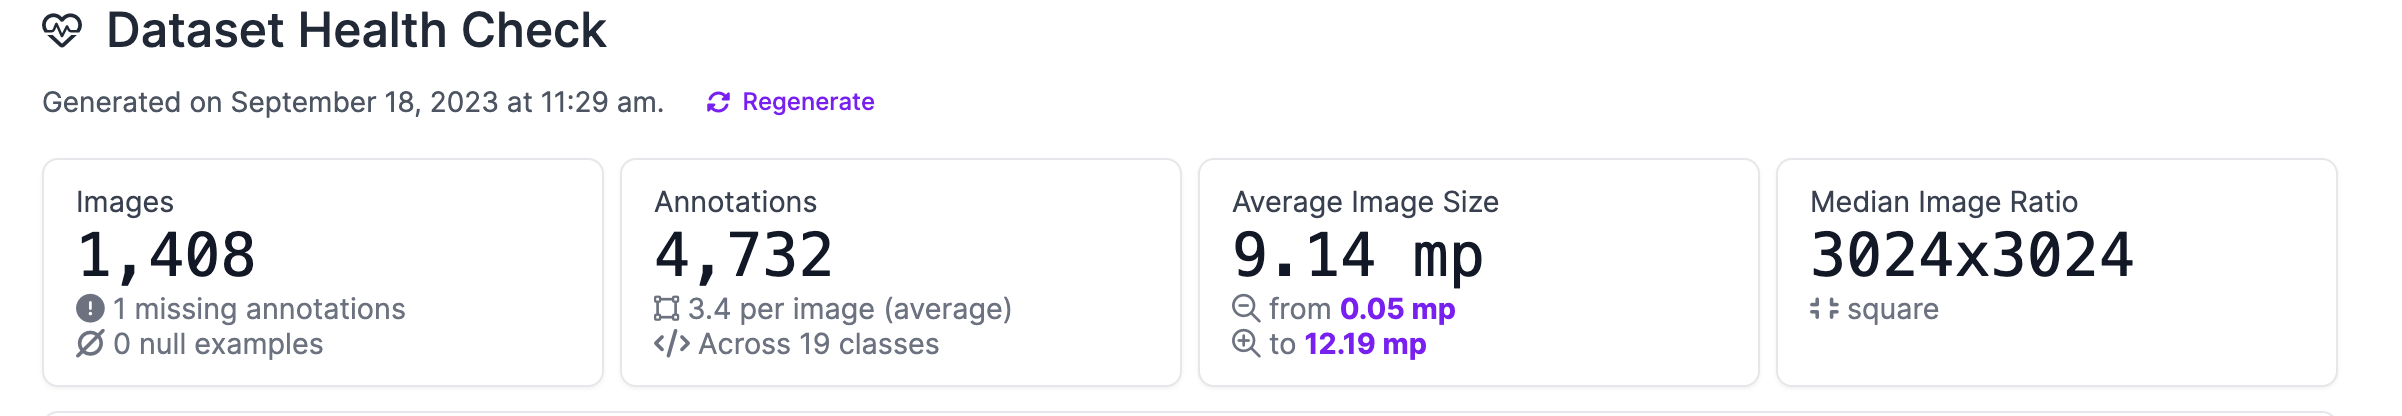
\includegraphics[width=0.45\textwidth]{figures/health.png}
  } \vfill
  \subfigure{
    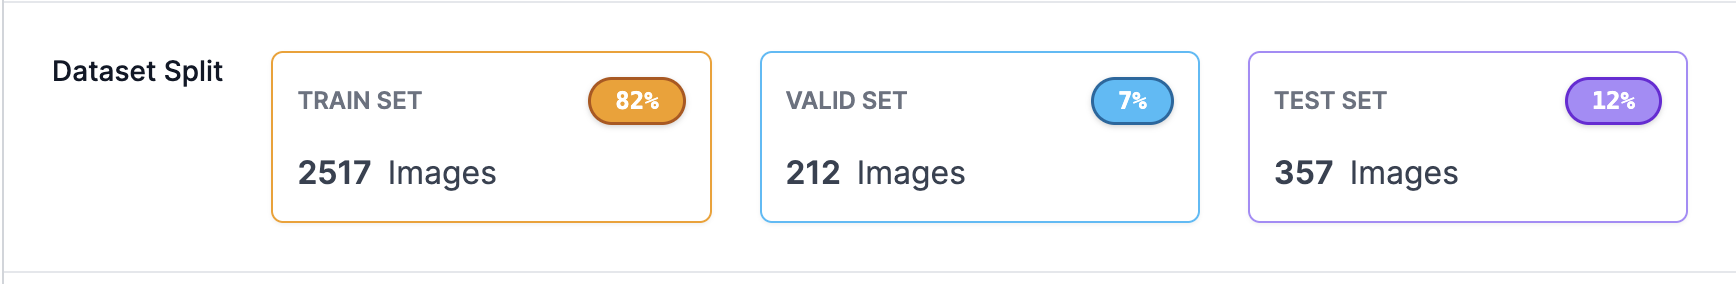
\includegraphics[width=0.45\textwidth]{figures/split.png}
  }
  \caption{Health check and train-test split of dataset}
  \label{fig:prob3-c}
\end{figure}


\subsection{Data Augmentation Methods}
Based on the Figure~\ref{fig:prob3-b}, the provided dataset uses the following augmentation steps:
\begin{enumerate}
  \item \textbf{Rotation (Between -15° and +15°):}
        \begin{itemize}
          \item Purpose: Rotating the images within a range of -15° to +15° helps the model become invariant to minor rotational changes.
          \item Usefulness: This is particularly useful for object detection in environments where the orientation of objects might vary slightly. For example, in a robotic setting where items might not always be perfectly aligned, the model needs to accurately identify objects regardless of their tilt.
        \end{itemize}
  \item \textbf{Bounding Box Noise (Up to 5\% of pixels):}
        \begin{itemize}
          \item Purpose: Adding noise to the bounding boxes simulates inaccuracies in bounding box annotations.
          \item Usefulness: This helps the model learn to tolerate slight inaccuracies in object localization, improving its robustness in detecting objects even when the bounding boxes are not perfectly annotated. This is crucial in real-world applications where perfect annotations are rare, and some level of noise is expected.
        \end{itemize}
\end{enumerate}

\begin{figure}[htbp]
  \centering
  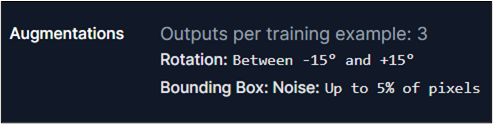
\includegraphics[width=0.45\textwidth]{figures/prob3-b.png}
  \caption{Augmentation methods used for \textit{Grasp\_6} dataset}
  \label{fig:prob3-b}
\end{figure}

\textbf{Detailed Explanation for Each Step:} \\
•	\textit{Rotation}: This augmentation mimics scenarios where the camera or objects might be slightly rotated. By training the model with rotated images, it can better handle real-world data where perfect alignment is not guaranteed. For instance, in a robotic vision system, the robot might encounter objects from various angles. Training with rotated images ensures the model can recognize these objects correctly despite the angle variations. \\
•	\textit{Bounding Box Noise}: This simulates the natural variance and potential errors in the bounding box annotations. In practical applications, bounding boxes might not be perfectly drawn around objects due to human error or automated annotation tools' limitations. Introducing noise helps the model become more resilient to such imperfections, ensuring that it can still perform well even when the bounding boxes are not perfectly accurate.
\vspace{10px}

\section{Problem 4: Object detection}
For this problem a \href{https://colab.research.google.com/drive/1RH5W2qrrn7r3mwXxXkabdknig7qeU1U5?usp=drive_link}{Jupyter Notebook} is created in \textit{Google Colab}. That's in order to utilize the Graphical Processing Unit that Google accommodates for high computational costly programs like training neural networks, such as the one in this problem. After training is done with 50 epochs, due to the GPU limits of Colab platform, we would save the trained weights in a \textit{Google Drive} directory and then switch to a normal unlimited CPU runtime. Then we can proceed the problem's demands via importing the saved model. We've chosen one of the latest YOLO versions for this problem: \underline{YOLO v8n}. As a result of this code, \textit{last.pt} and \textit{best.pt} files, which contain the trained weights of the network, are generated in \texttt{YOLOv8\_training/exp-13/weights} directory. In addition, some pictures are saved to demonstrate the difference between the model's predictions and the true labels of some objects (Figure~\ref{fig:prob4-a}). Although the results are satisfying, the model is unable to predict some objects, or predicts them with wrong labels at this stage. The evaluation metrics like different losses or mAP scores are also saved in a csv file, while their promising trends are plotted in Figure~\ref{fig:prob4-b}. The obtained confusion matrix also has maximum and close to 1 values on its main diagonal and thus, seems promising (Figure~\ref{fig:prob4-c}). Some other monitoring specs are also generated that are not of much importance in this project (Figure~\ref{fig:prob4-d}). As a final result, the model's prediction on unknown test images provided in a separate Drive is shown in Figure~\ref{fig:prob4-e}, which announces almost fully accurate results.

\subsection*{Training Report Explanation}

When I trained a YOLOv8n (a variant of the YOLOv8 model) on the dataset, the training process generated a detailed report summarizing various performance metrics and other relevant information about the model's learning progress. This report typically includes several tables and plots that help to understand how well the model performed during training and validation. Here is an explanation of the key components found in the training report:

\subsubsection*{1. Training and Validation Metrics}
These metrics are often presented in tabular format and include:
\begin{itemize}
  \item \textbf{Precision:} The ratio of true positive detections to the total number of positive predictions (true positives + false positives). It measures the accuracy of the positive predictions made by the model.
  \item \textbf{Recall:} The ratio of true positive detections to the total number of actual positives (true positives + false negatives). It measures the model's ability to detect all relevant objects.
  \item \textbf{mAP (mean Average Precision):} A common metric in object detection, it averages the precision across different recall levels. It's often computed at different Intersection over Union (IoU) thresholds, such as mAP@0.5 and mAP@0.5:0.95.
  \item \textbf{F1 Score:} The harmonic mean of precision and recall, providing a single metric that balances the two.
  \item \textbf{Loss:} This is a measure of how well the model is performing during training. The loss function combines multiple components such as classification loss, localization loss, and objectness loss.
\end{itemize}

\subsubsection*{2. Loss Curves}
These are plots showing how the loss changes over epochs for both the training and validation datasets. Typically, you would see:
\begin{itemize}
  \item \textbf{Training Loss Curve:} This plot shows the loss on the training dataset as the training progresses. Ideally, this should decrease over time as the model learns from the data.
  \item \textbf{Validation Loss Curve:} This plot shows the loss on the validation dataset. This is crucial for understanding whether the model is overfitting (validation loss increases while training loss decreases) or underfitting (both losses are high).
\end{itemize}

\subsubsection*{3. Precision-Recall Curve}
A plot of precision versus recall for different thresholds. It helps to visualize the trade-off between precision and recall for different confidence thresholds. The area under this curve is related to the mAP.

\subsubsection*{4. Confusion Matrix}
A matrix that shows the number of true positive, false positive, true negative, and false negative predictions. This is particularly useful for understanding where the model is making errors.

\subsubsection*{5. Learning Rate Schedule}
A plot or table showing how the learning rate changes over epochs. Understanding the learning rate schedule can help diagnose issues with convergence or instability during training.

\subsubsection*{6. Inference Results}
Some training reports may include examples of inference results on a subset of validation images. These can help qualitatively assess how well the model is performing.

\subsection*{Why Does the Model Get Some Outputs Wrong?}

The model showed acceptable performance both on training and validation/test sets; yet it might produce incorrect outputs due to several reasons:

\begin{itemize}
  \item \textbf{Insufficient Training Data:} The model may not have seen enough examples of certain objects or scenarios during training.
  \item \textbf{Imbalanced Dataset:} If some classes are underrepresented, the model might not learn to detect them accurately.
  \item \textbf{Overfitting:} The model might perform well on training data but poorly on new, unseen data.
  \item \textbf{Noise and Variability:} Variations in lighting, occlusion, and background clutter can confuse the model.
  \item \textbf{Ambiguity in Labels:} Inconsistent or incorrect labeling in the training dataset can mislead the model.
  \item \textbf{Model Complexity:} The model might be too simple to capture complex patterns in the data, or too complex, leading to overfitting.
  \item \textbf{Suboptimal Hyperparameters:} Incorrect settings for learning rate, batch size, and other hyperparameters can hinder the model's learning process.
\end{itemize}


\begin{figure}[htbp]
  \centering
  \subfigure[True Labels - sample 1]{
    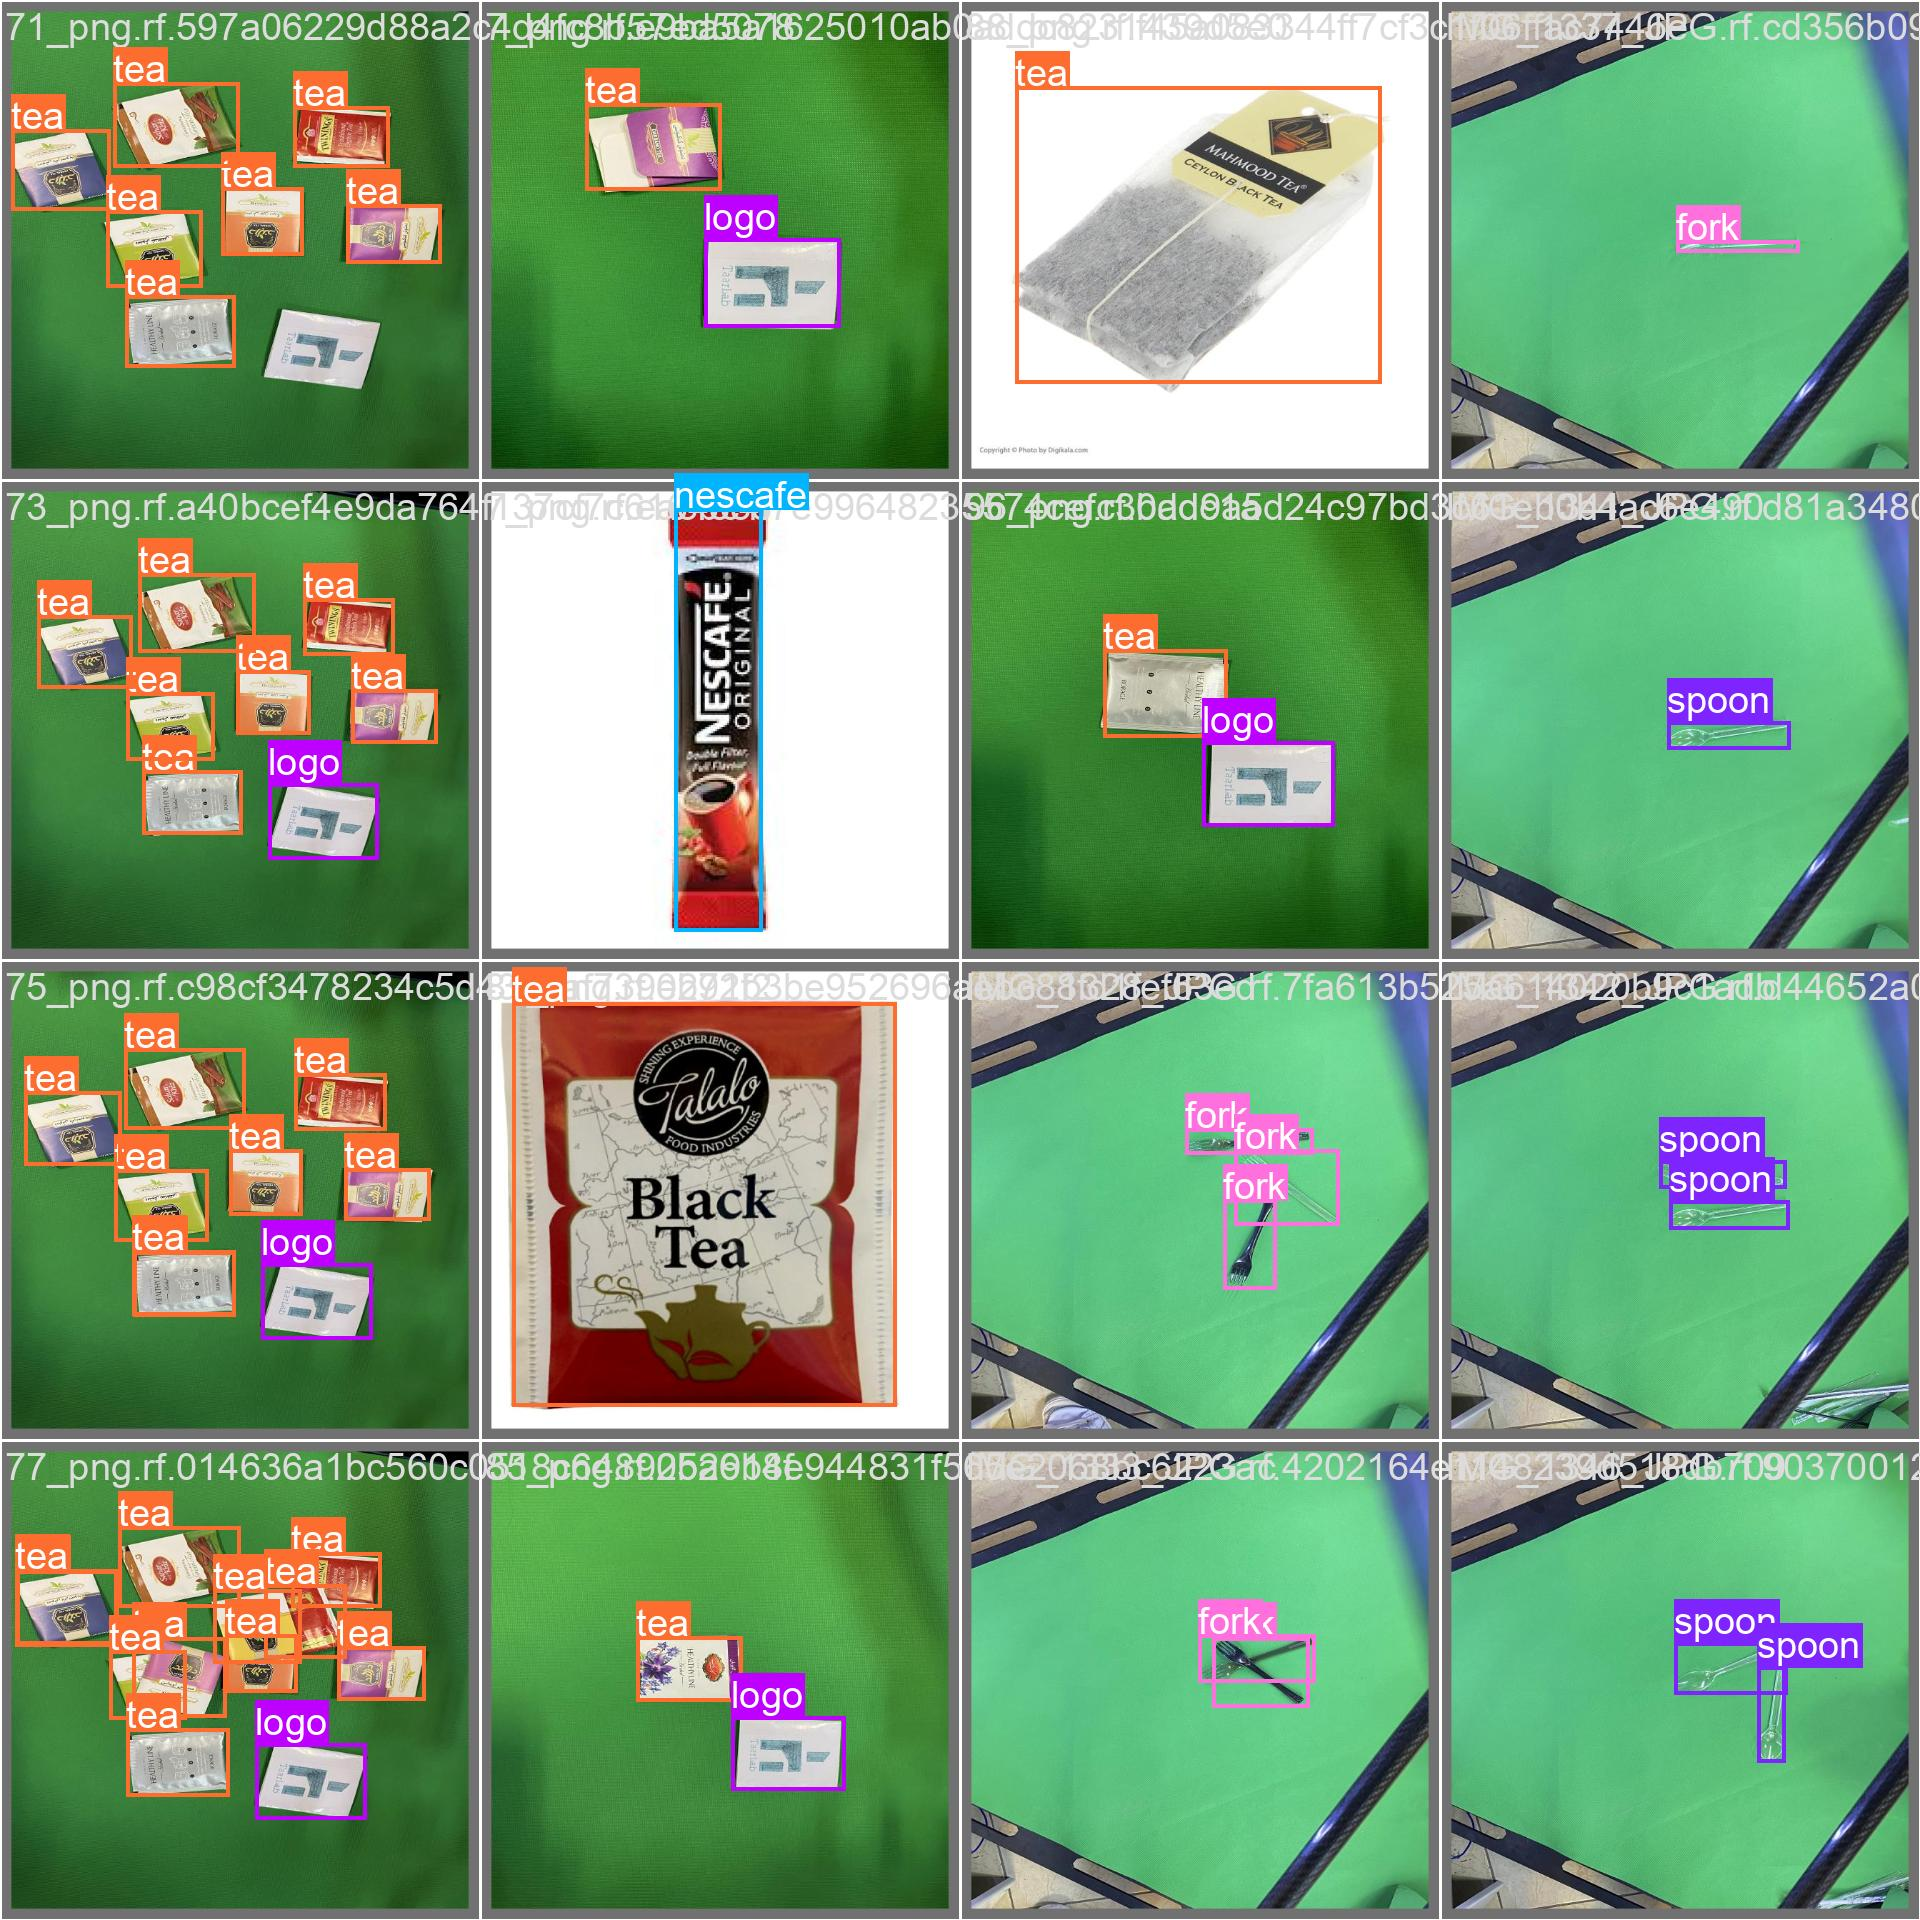
\includegraphics[width=0.22\textwidth]{figures/val_batch2_labels.jpg}
    \label{fig:subfig1}
  } \hfill
  \subfigure[Model's Prediction - sample 1]{
    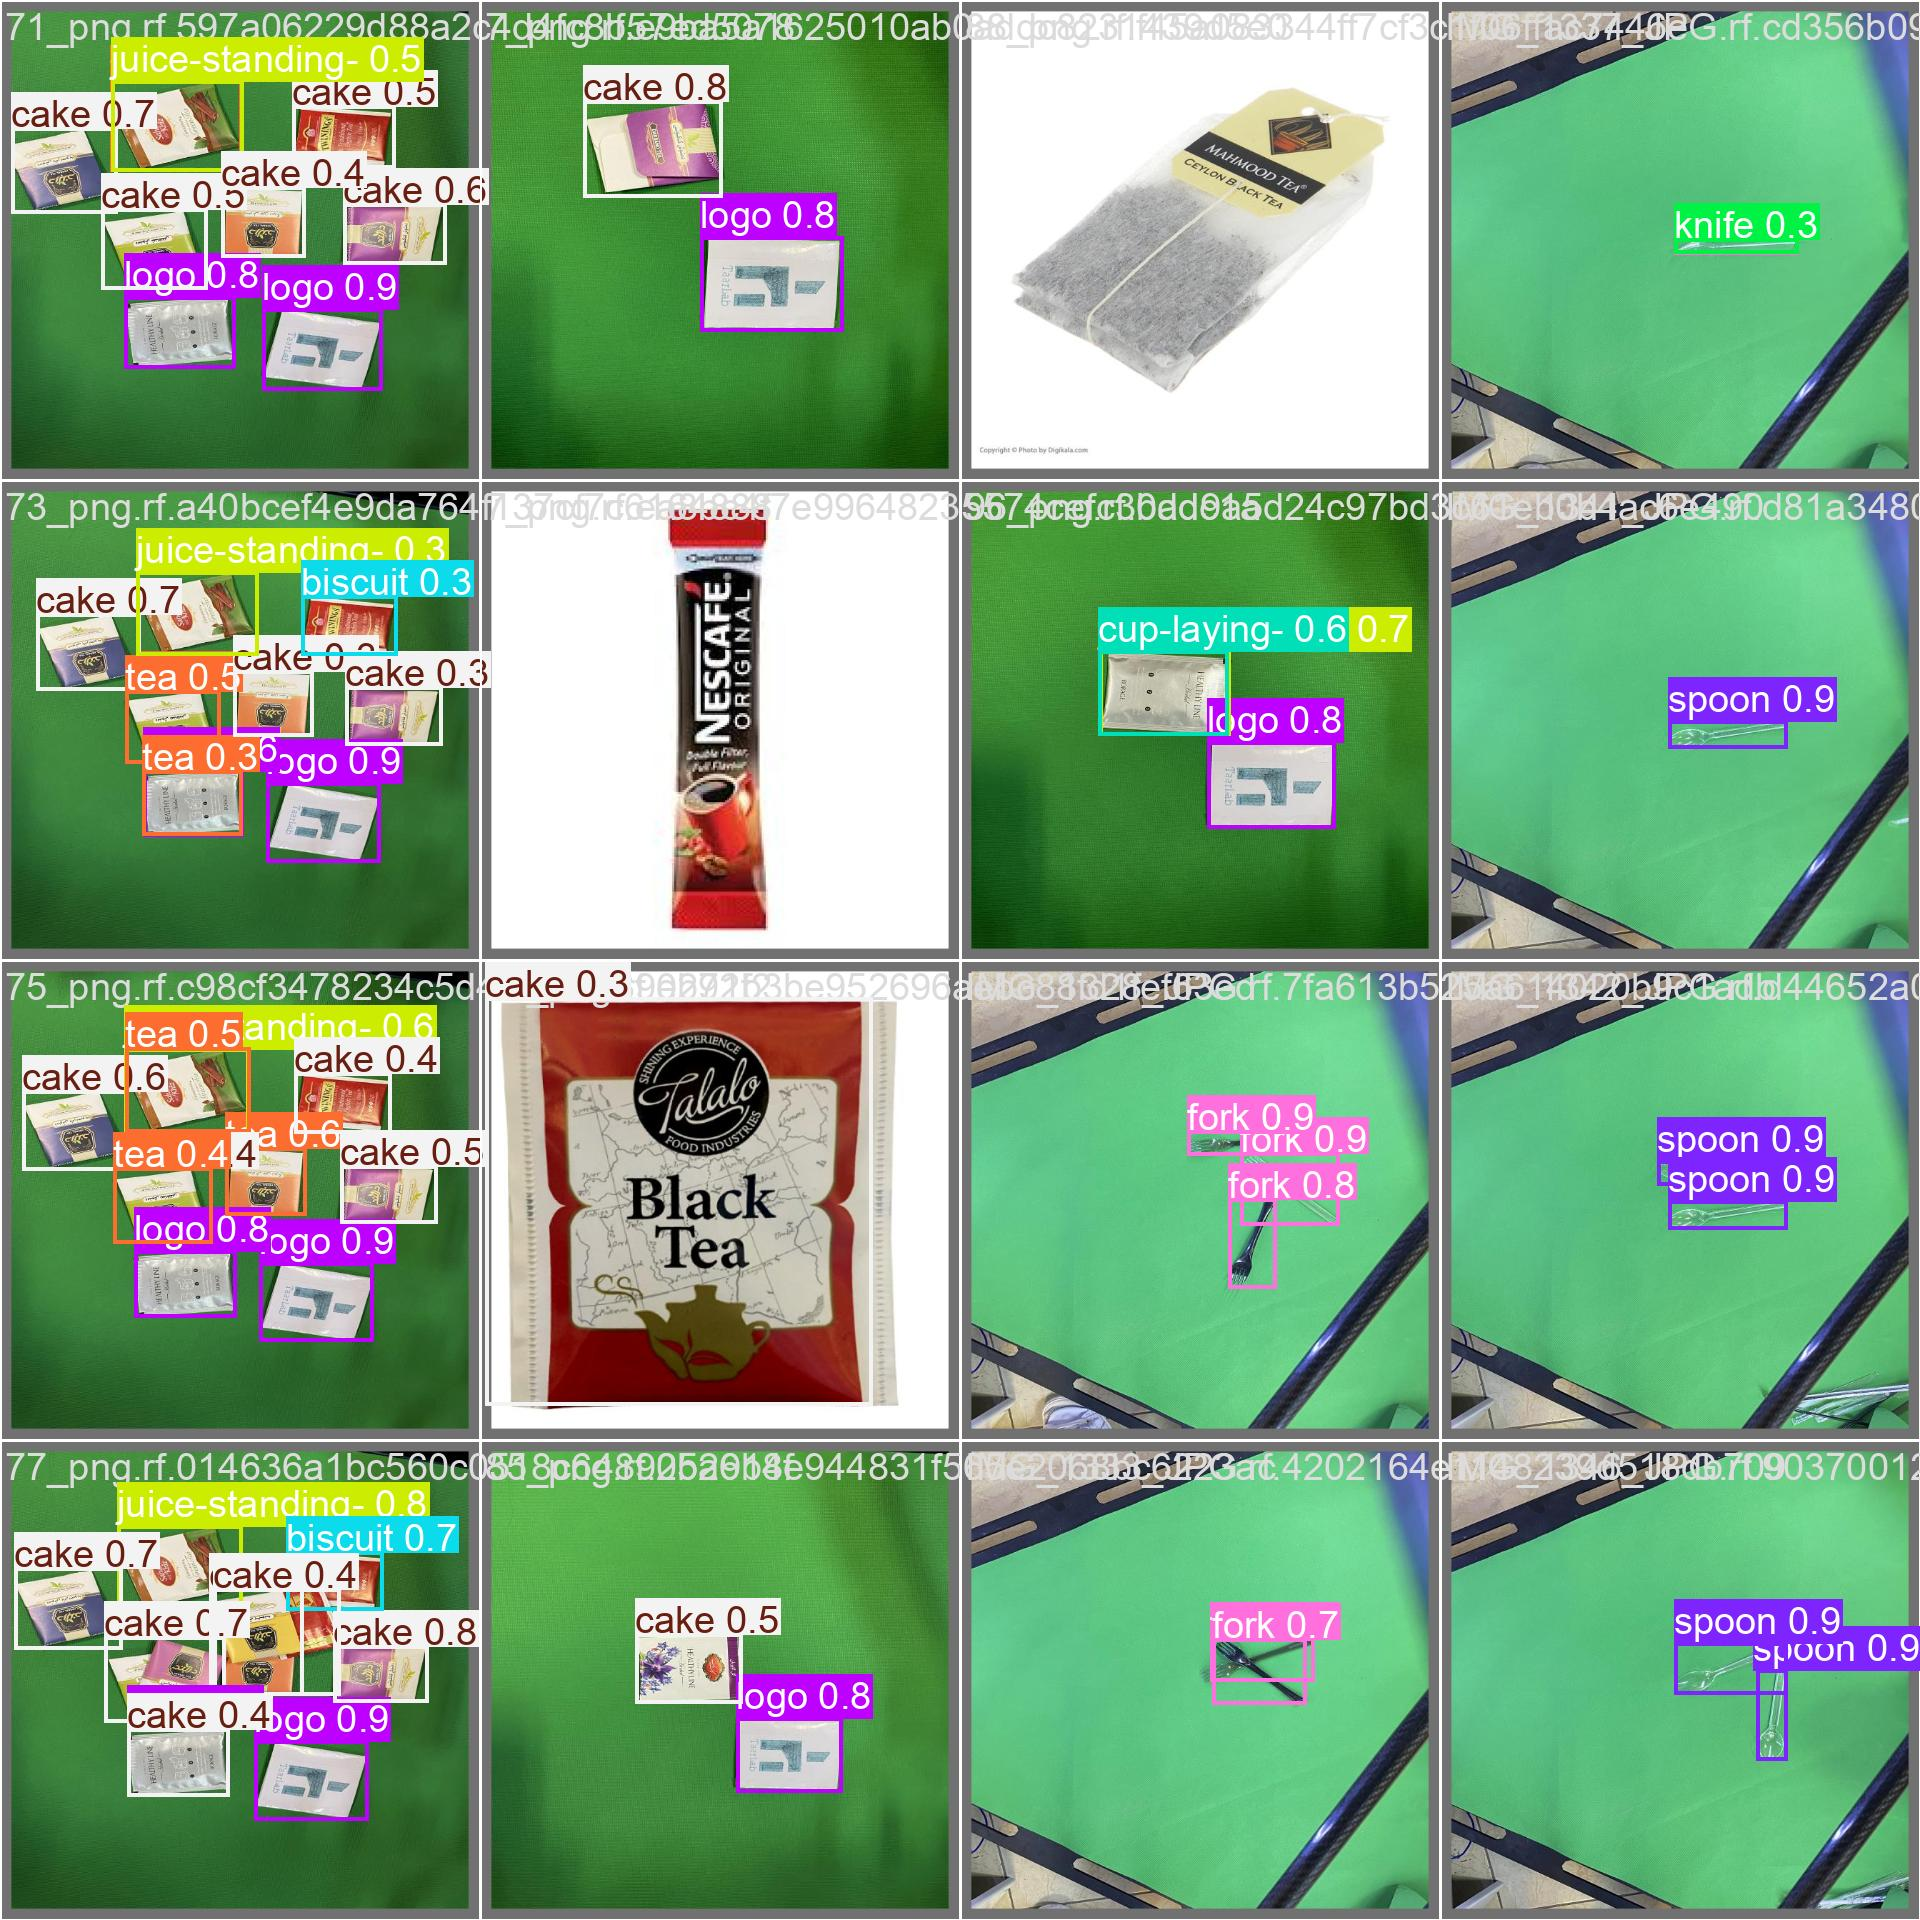
\includegraphics[width=0.22\textwidth]{figures/val_batch2_pred.jpg}
    \label{fig:subfig2}
  } \vfill
  \subfigure[True Labels - sample 2]{
    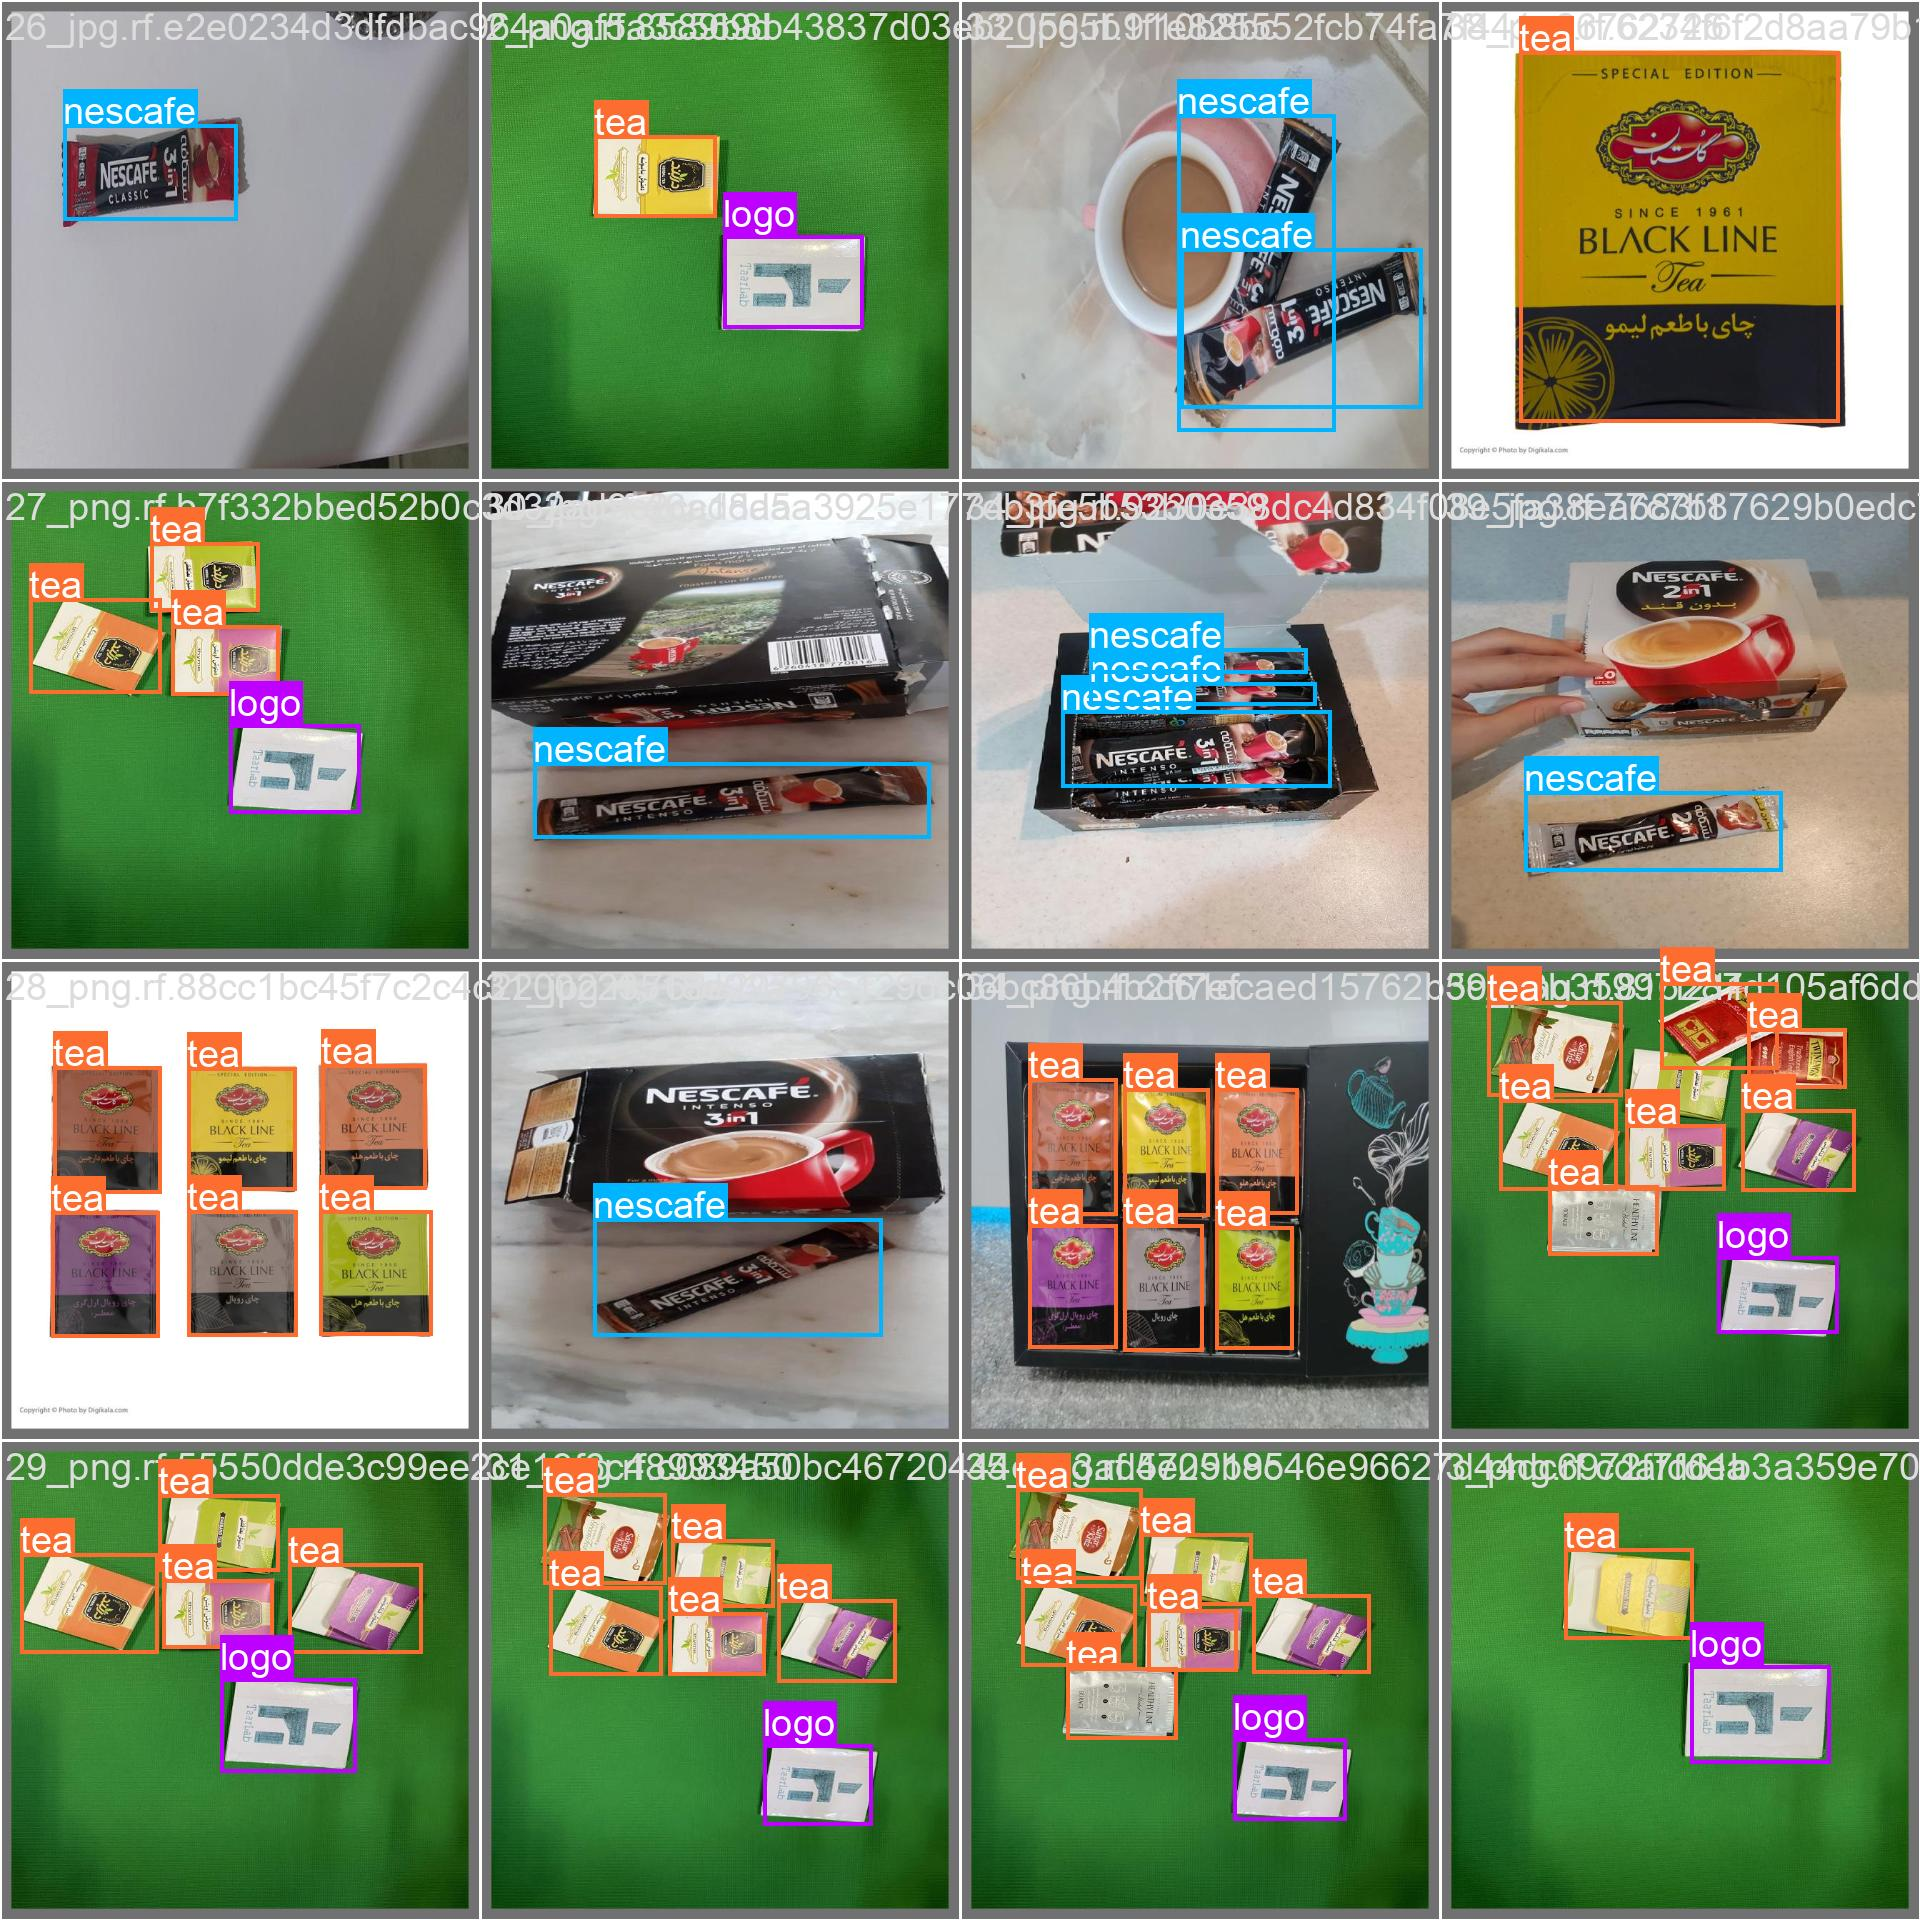
\includegraphics[width=0.22\textwidth]{figures/val_batch1_labels.jpg}
    \label{fig:subfig3}
  } \hfill
  \subfigure[Model's Prediction - sample 2]{
    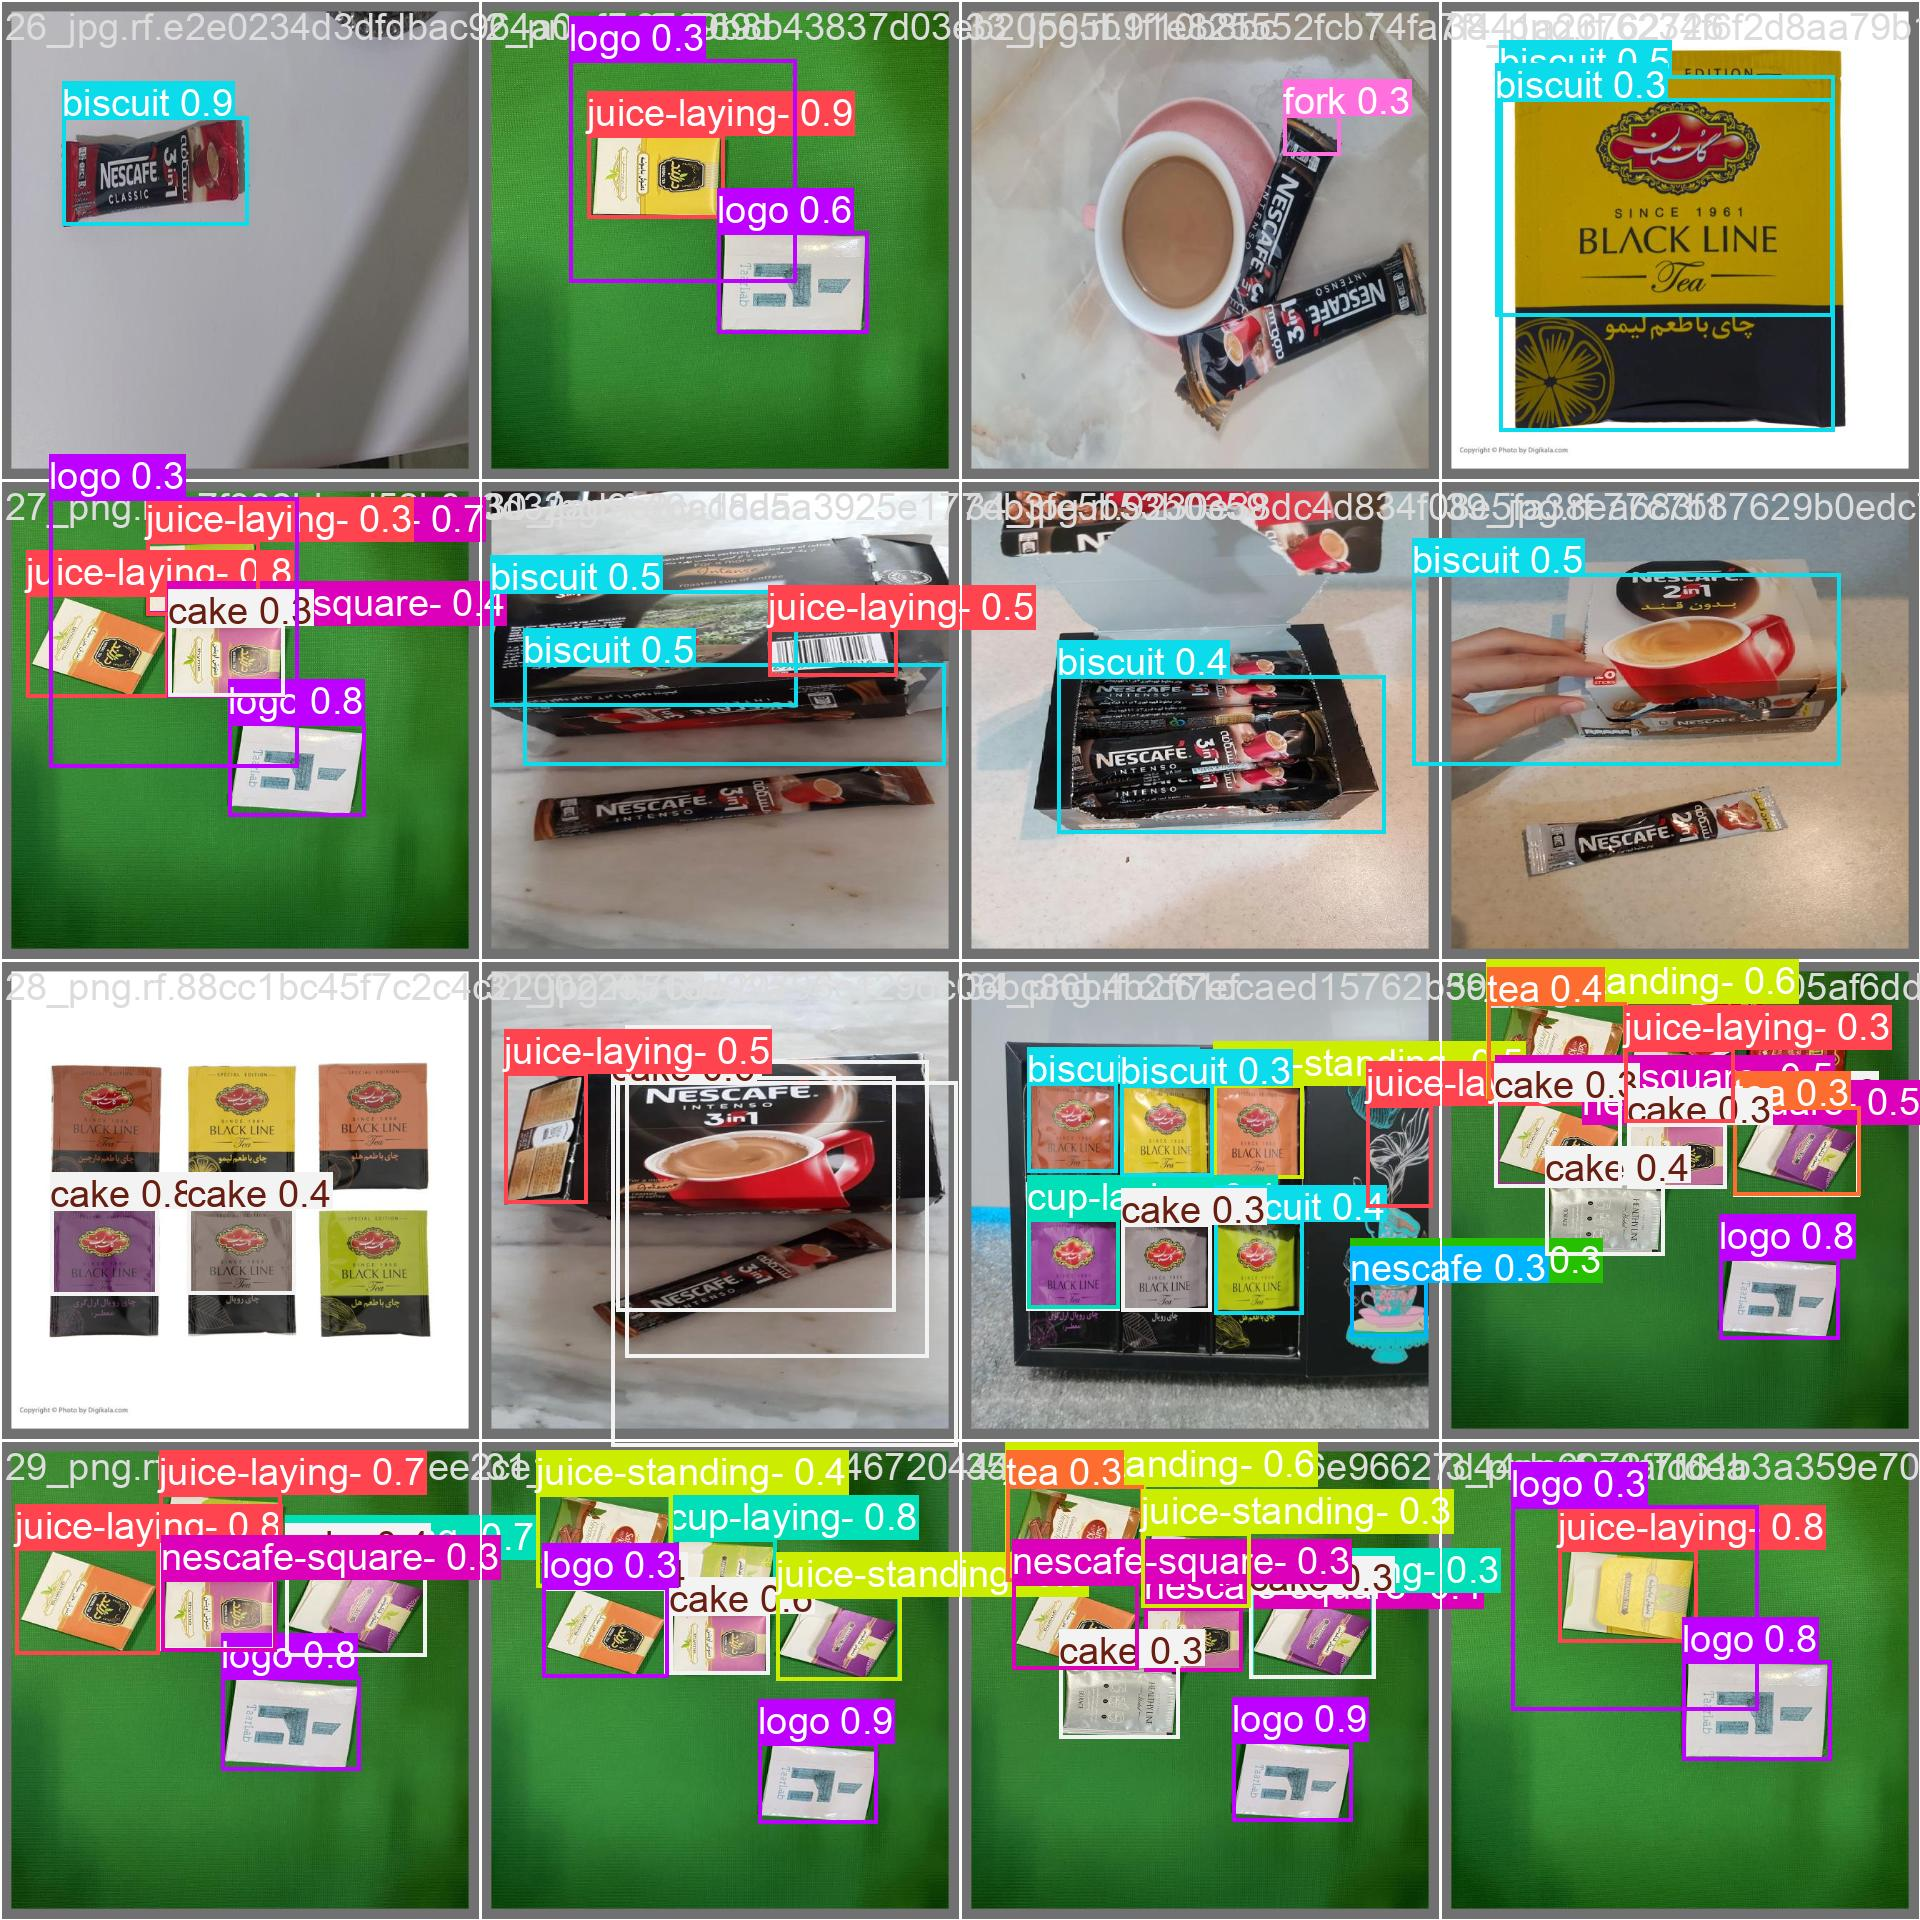
\includegraphics[width=0.22\textwidth]{figures/val_batch1_pred.jpg}
    \label{fig:subfig4}
  }
  \caption{Comparison between predicted and true labels of different objects}
  \label{fig:prob4-a}
\end{figure}

\begin{figure}[htbp]
  \centering
  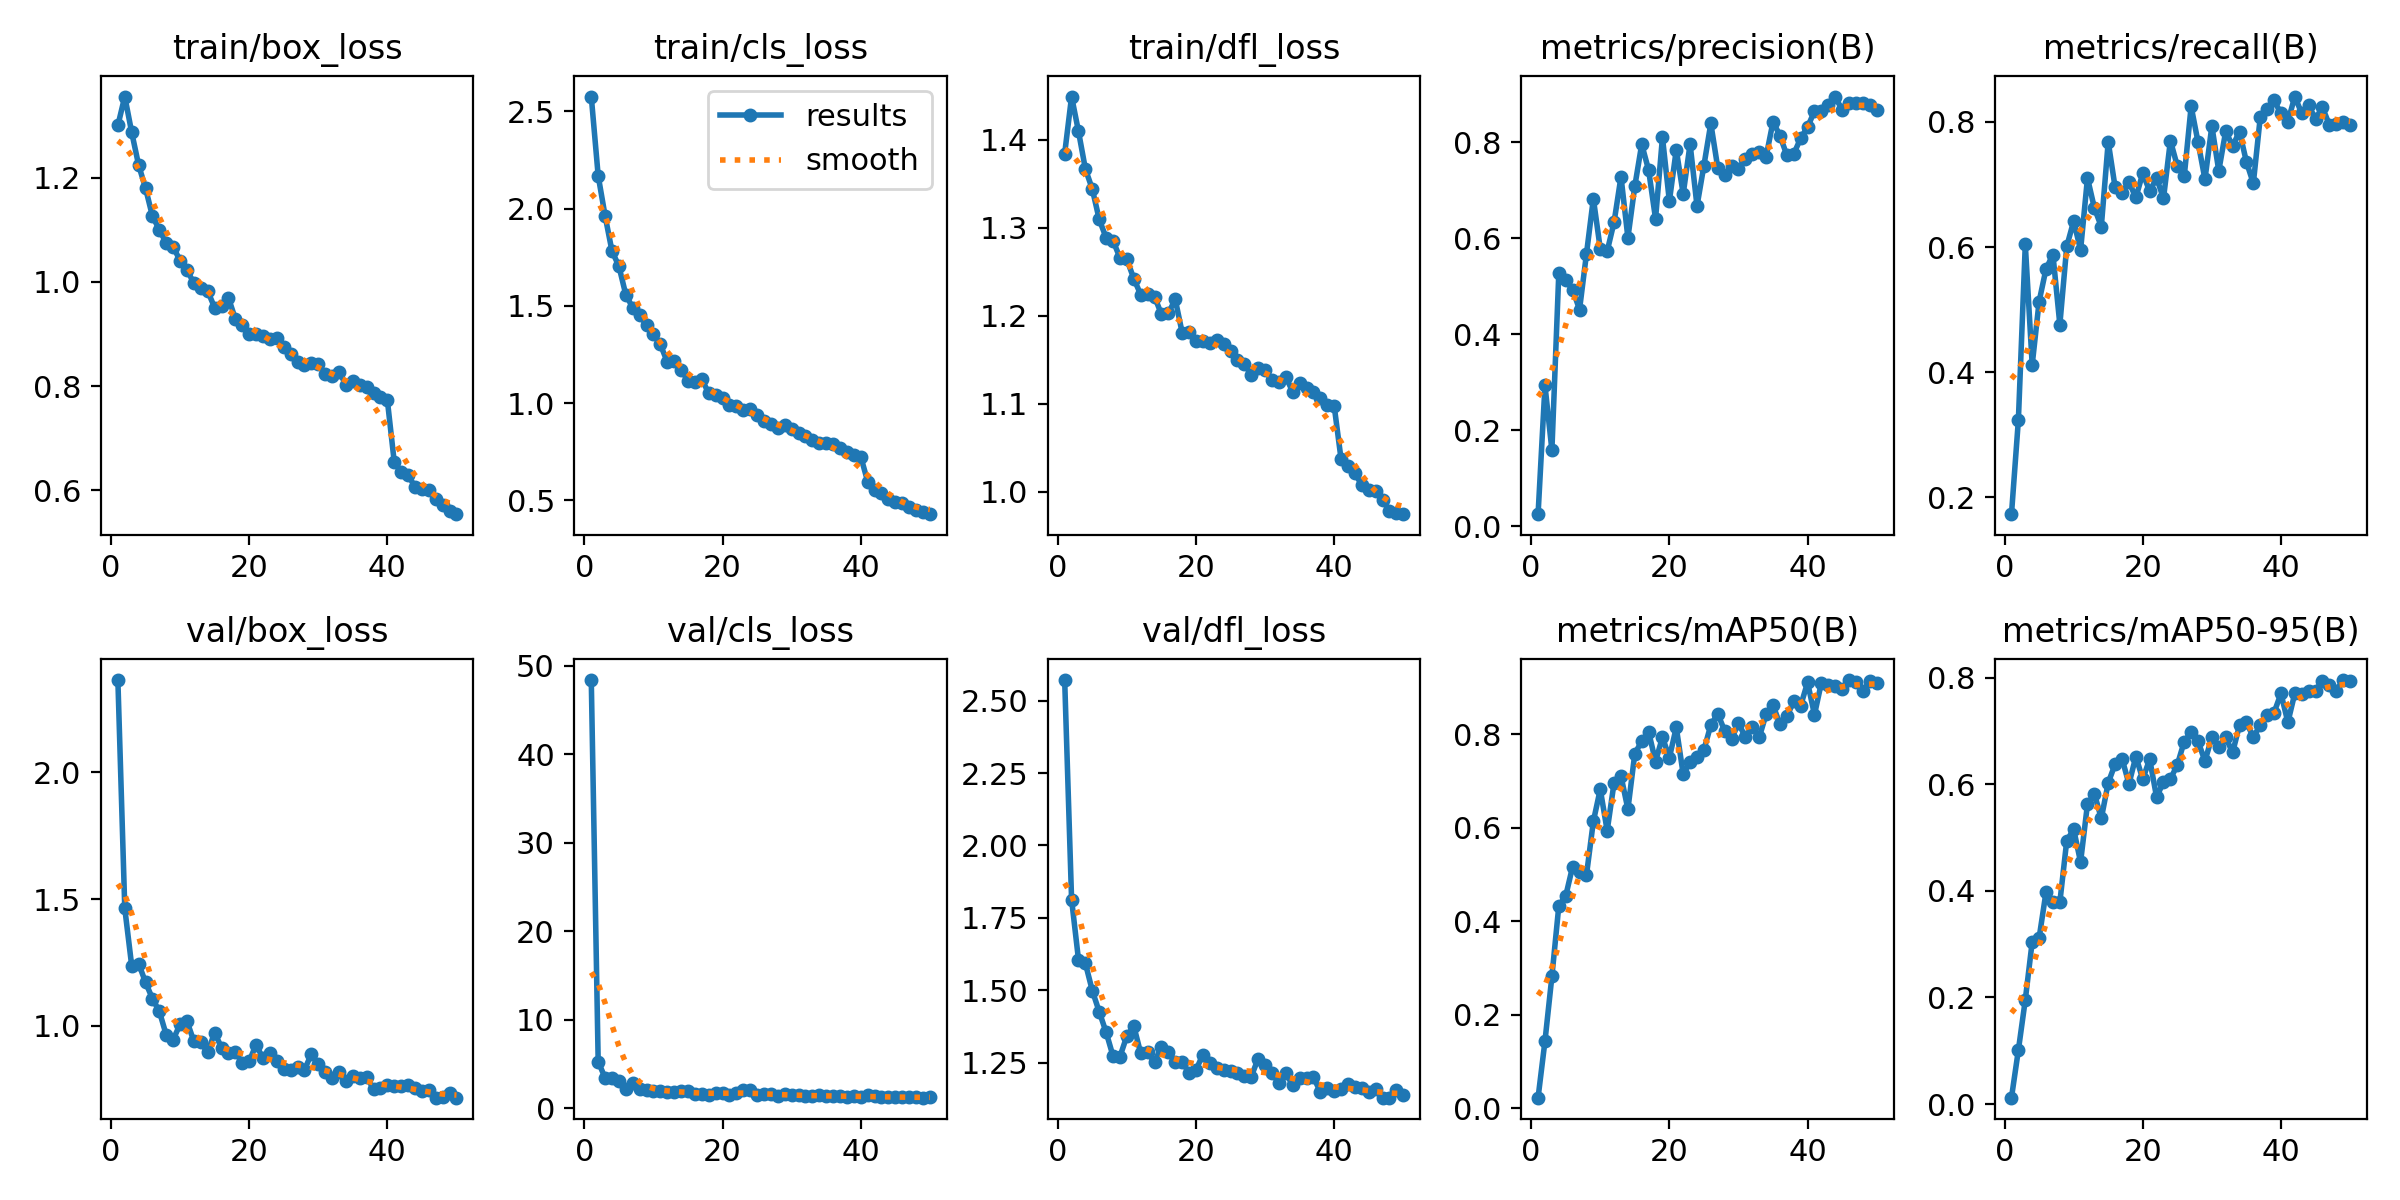
\includegraphics[width=0.44\textwidth]{figures/results.png}
  \caption{Loss, Precision, Recall and mAP metrics of the model}
  \label{fig:prob4-b}
\end{figure}

\begin{figure}[htbp]
  \centering
  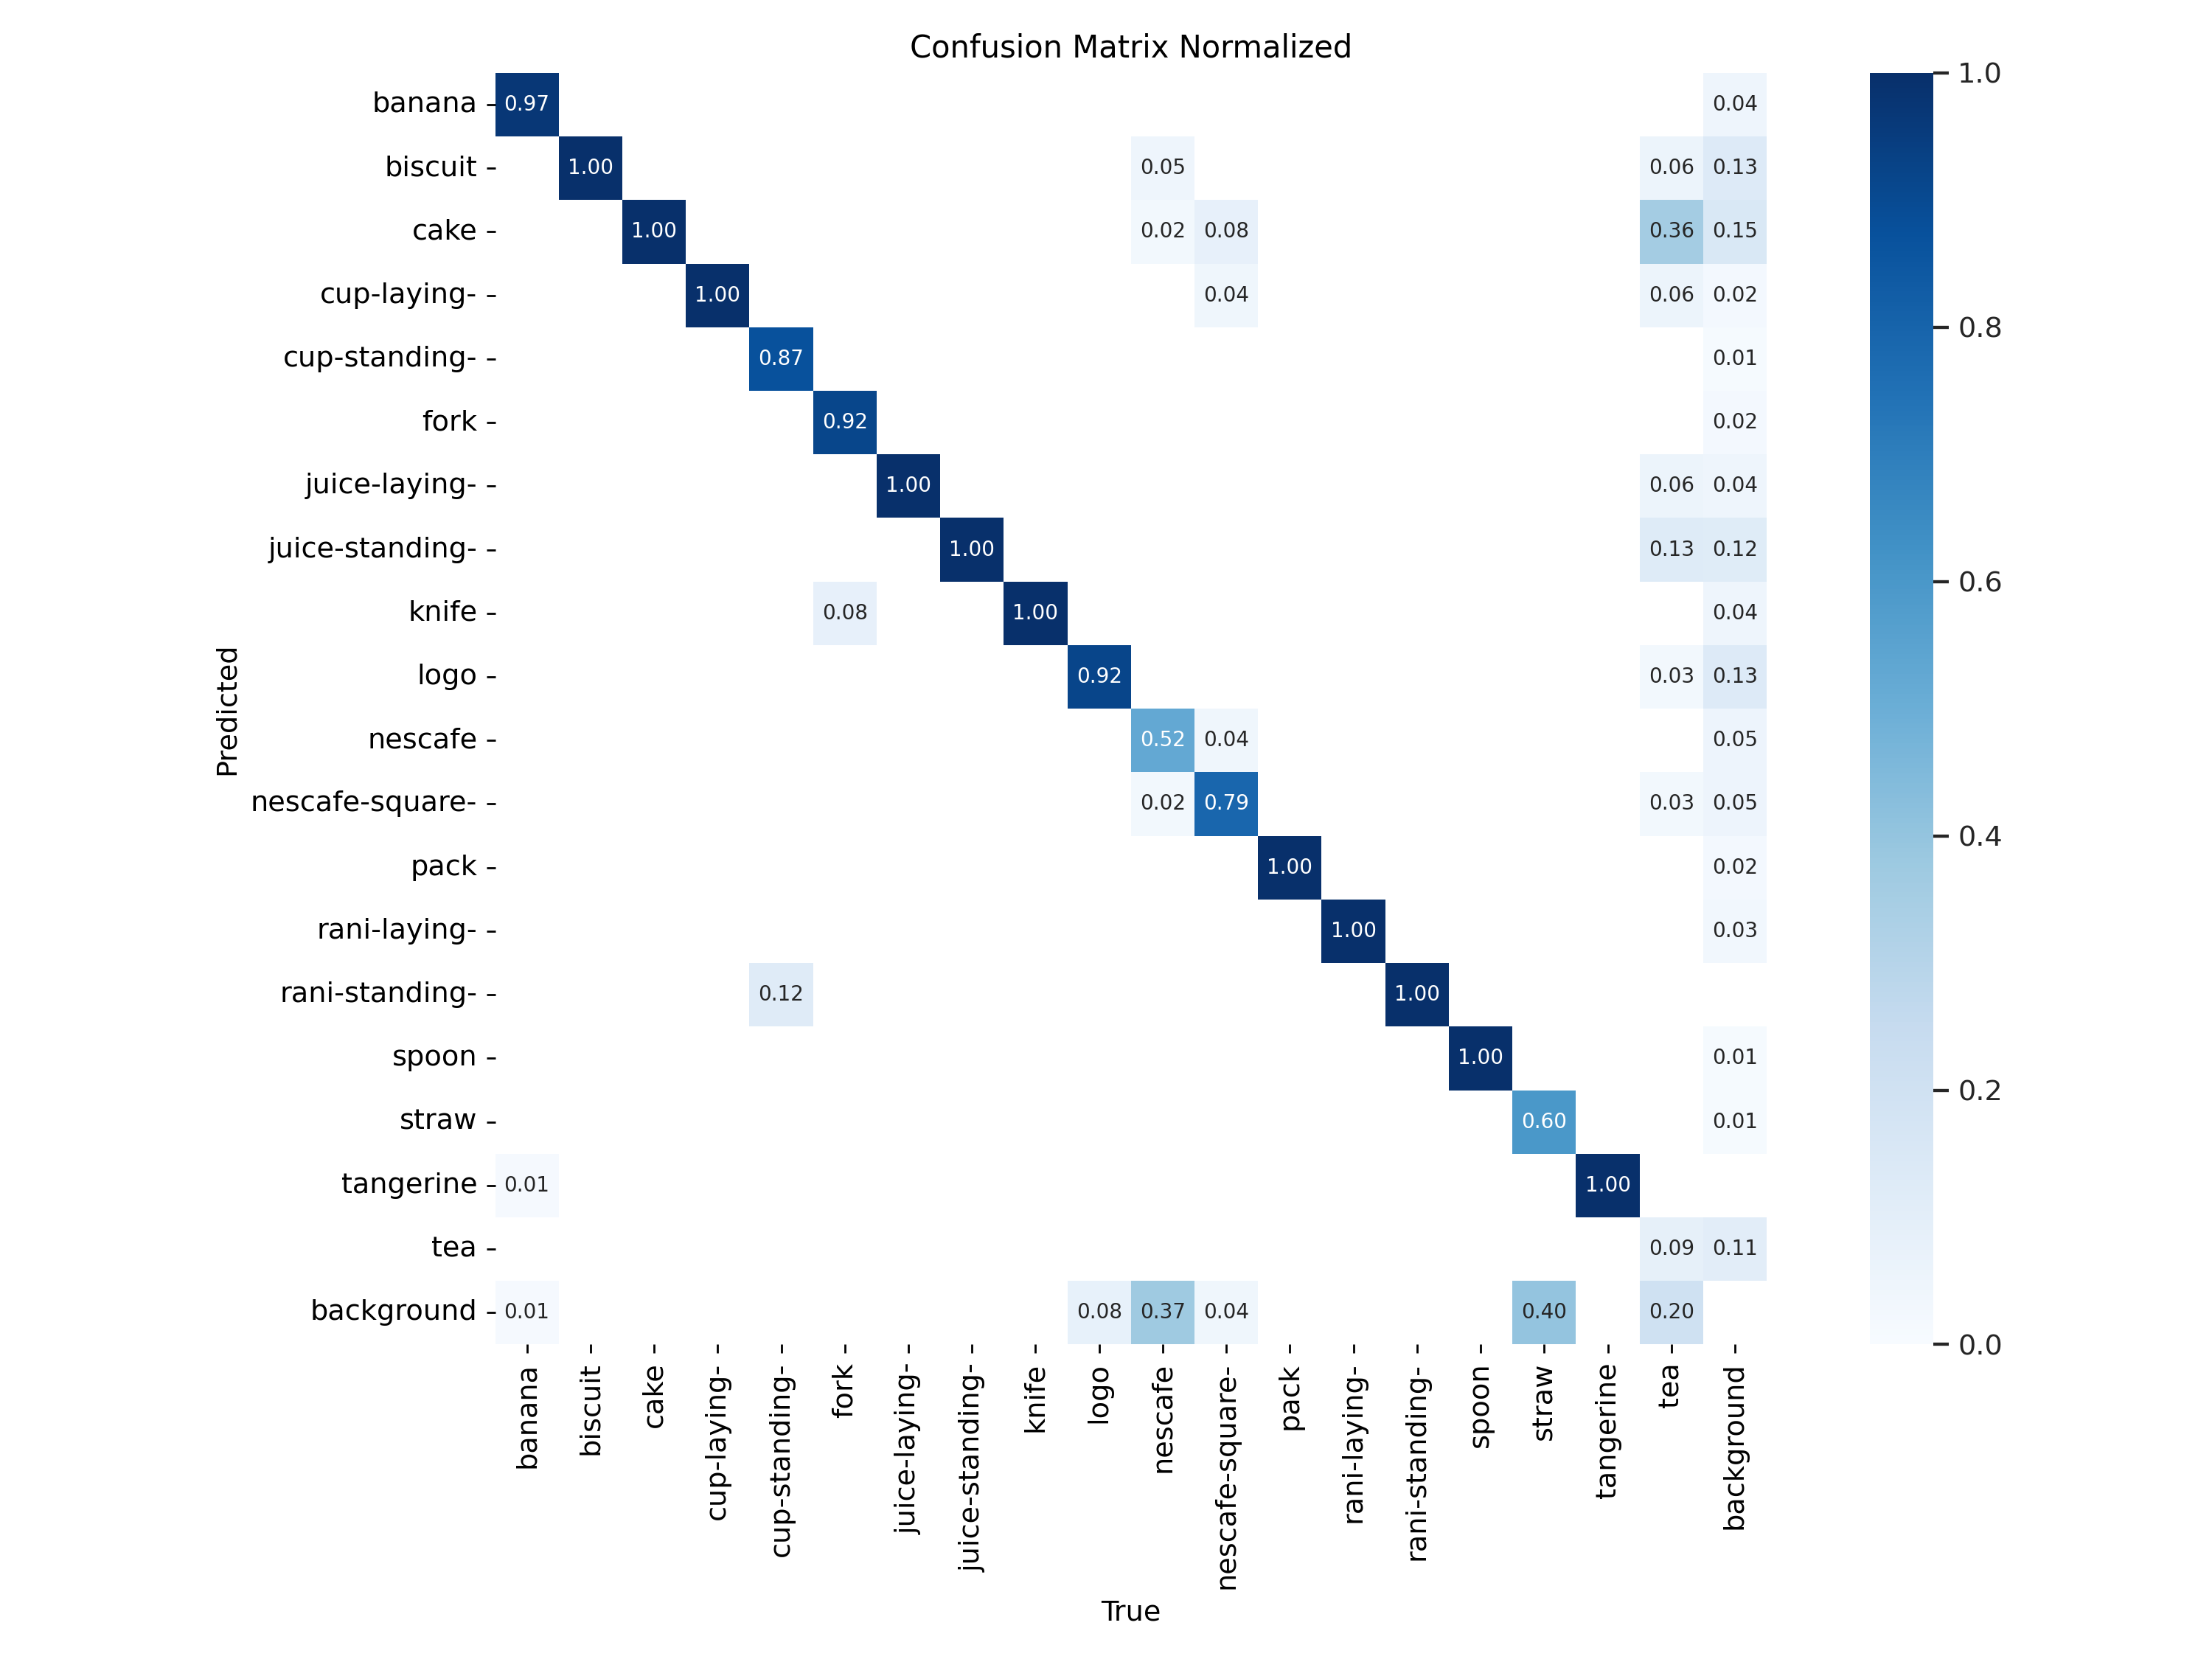
\includegraphics[width=0.5\textwidth]{figures/confusion_matrix_normalized.png}
  \caption{Normalized Confusion Matrix of the model}
  \label{fig:prob4-c}
\end{figure}

\begin{figure}[htbp]
  \centering
  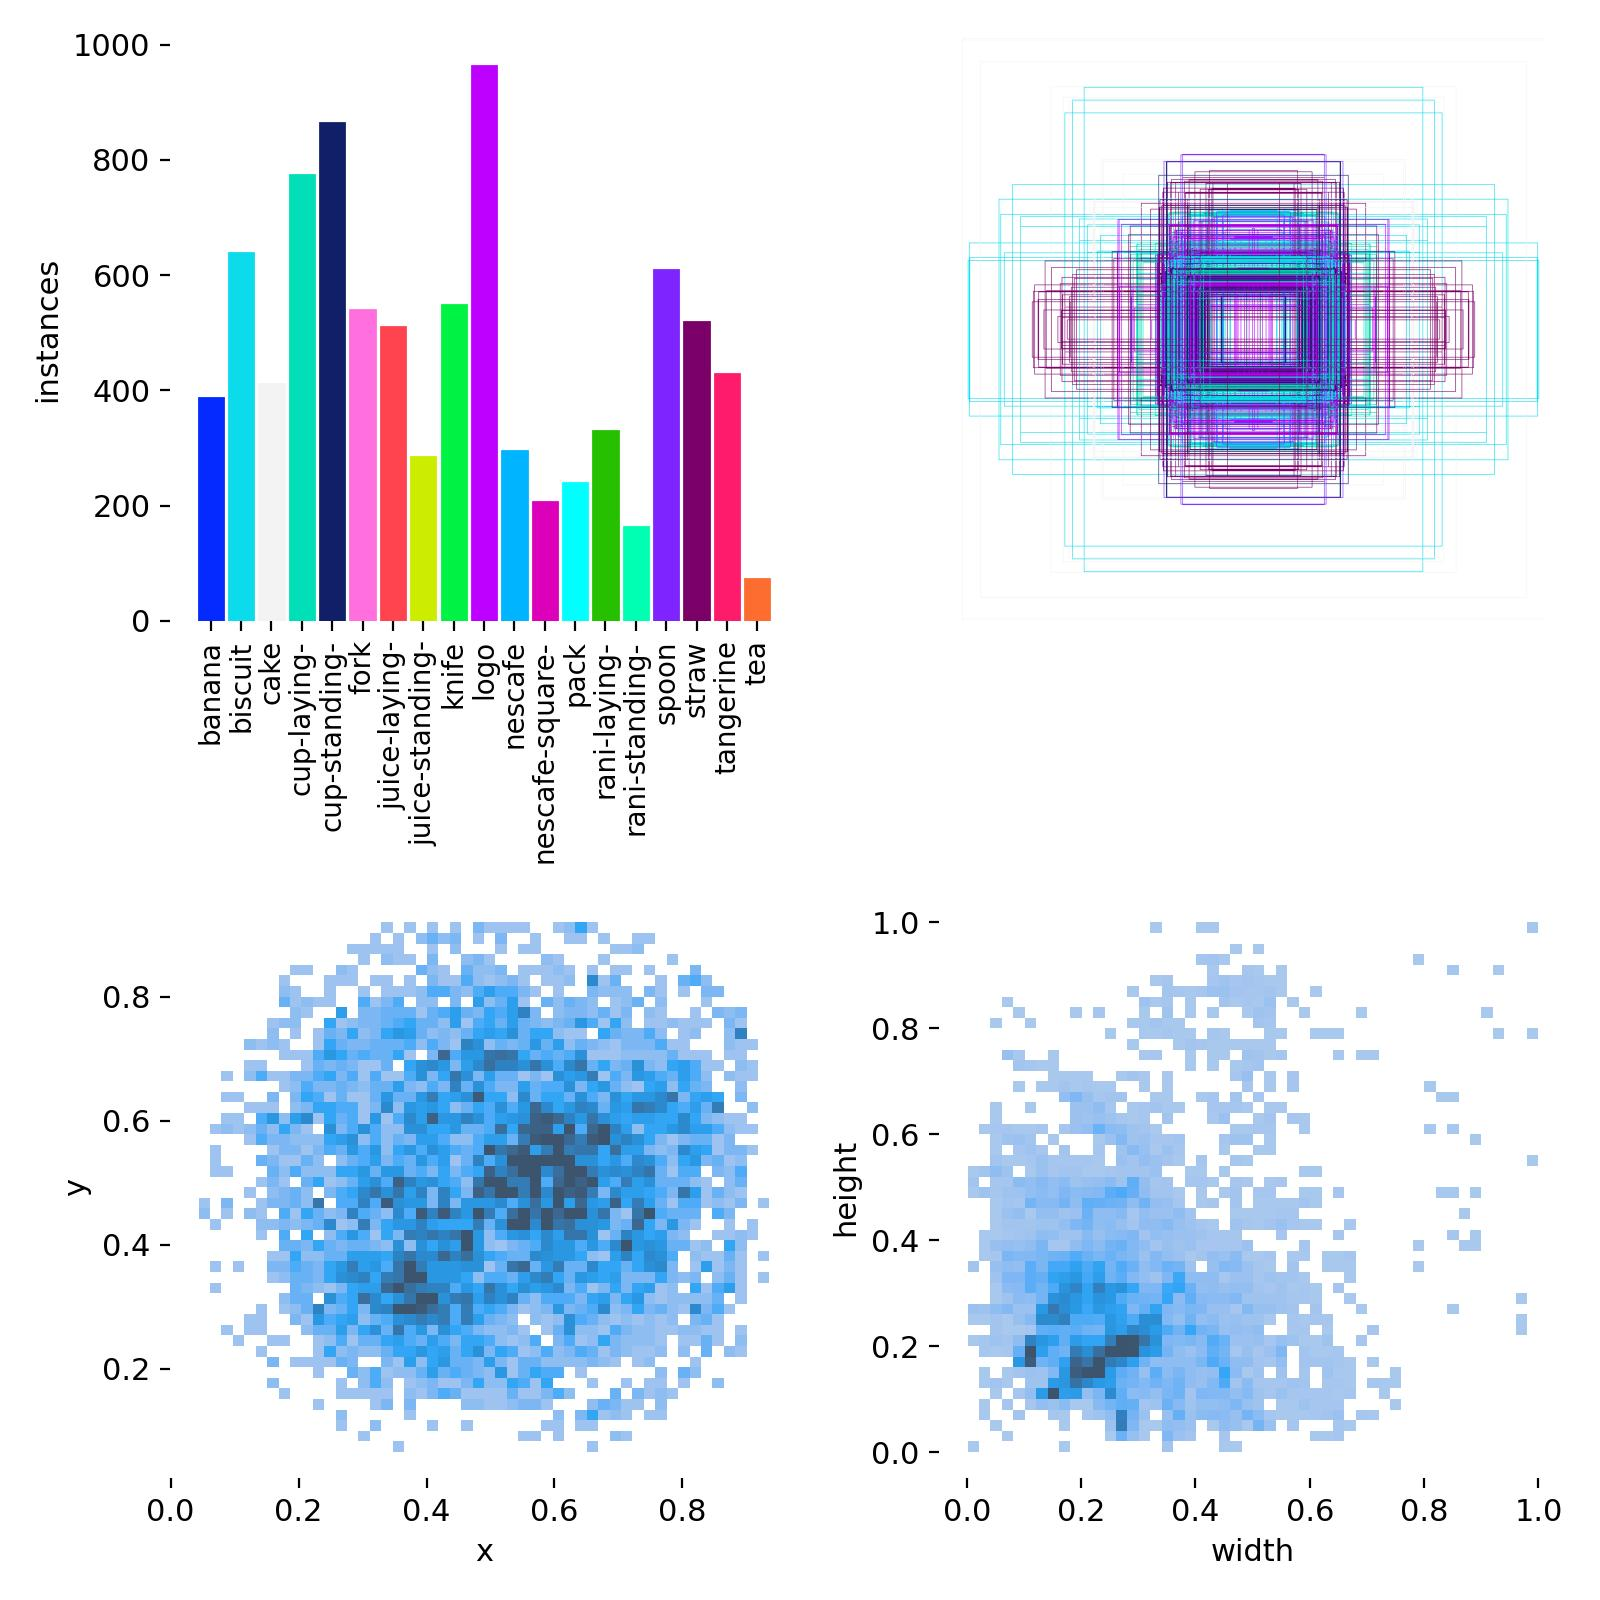
\includegraphics[width=0.45\textwidth]{figures/labels.jpg}
  \caption{Class Distribution and dataset info}
  \label{fig:prob4-d}
\end{figure}

\begin{figure}[htbp]
  \centering
  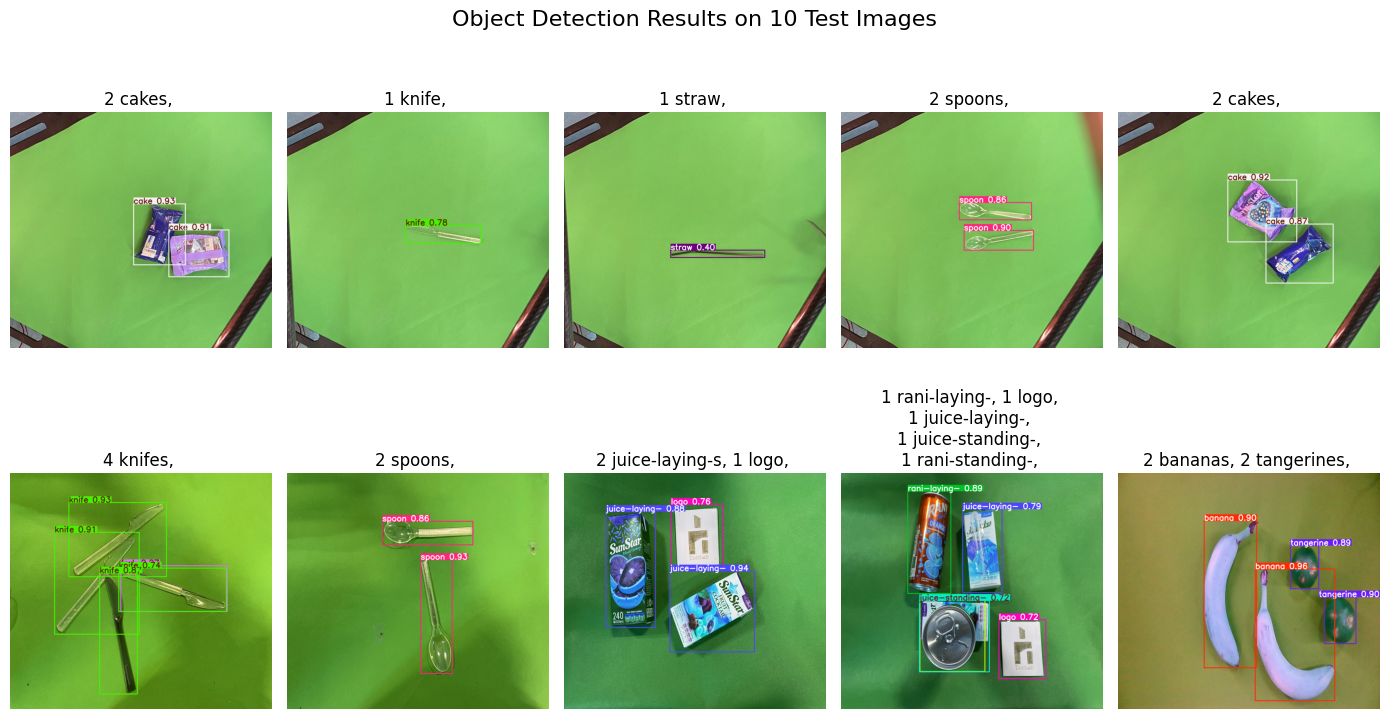
\includegraphics[width=0.49\textwidth]{figures/prob4.png}
  \caption{Object detection on 10 test images via YOLO v8}
  \label{fig:prob4-e}
\end{figure}
\vspace{10px}

\section{Problem 5: Object segmentation}
\subsection{Object detection vs. Object segmentation}
Object detection and segmentation are both techniques used in computer vision but serve different purposes. Object detection involves identifying and locating objects within an image by providing bounding boxes around each detected object and class labels indicating what the objects are. In contrast, segmentation involves partitioning an image into regions corresponding to different objects or classes, offering pixel-level detail. There are two types of segmentation: semantic segmentation, which classifies each pixel into a category without distinguishing between instances of the same class, and instance segmentation, which classifies each pixel while also distinguishing between different instances of the same class.

\subsection{FastSAM vs. YOLO}
FastSAM is a segmentation model designed for efficient and accurate object segmentation tasks. Unlike YOLO, which focuses on object detection by identifying and locating objects with bounding boxes and class labels, FastSAM provides pixel-level segmentation, identifying the exact boundaries of objects within an image.
FastSAM is used for object segmentation by taking an input image and producing a segmentation mask for each object. This mask delineates the precise pixels belonging to each object, allowing for more detailed and fine-grained analysis compared to object detection. This capability makes FastSAM suitable for applications requiring high spatial resolution, such as medical imaging, autonomous driving, and image editing.

\subsection{Implementation of FastSAM}
For this problem a \href{https://colab.research.google.com/drive/1I6auu-cPE4nA_uiOiNw0u5TZJ6KCrFXq#scrollTo=tIgKnKD8Cv51}{Jupyter Notebook} is created in \textit{Google Colab}. Despite all of the authors' attempts, installing and importing \textit{FastSAM} using direct \texttt{pip} commands were nothing but failure. To address this problem, some web searches \cite{b5} have inspired the program which installs and clones the required packages mainly from \textit{Github}. Going through these installations, imports and initializations, we've become able to re-use the previous boundary boxes drawn on the test images via YOLO model, to apply FastSAM model and conduct precise object segmentation task with creating masks. The final result can be seen in Figure~\ref{fig:prob5}.

\begin{figure}[htbp]
  \centering
  \subfigure{
    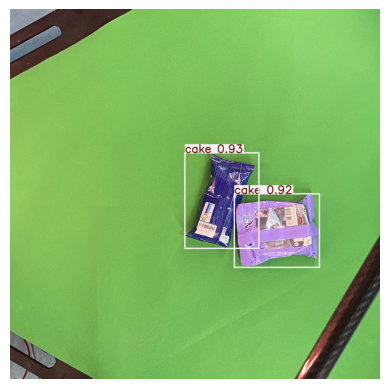
\includegraphics[width=0.21\textwidth]{figures/prob4-1.png}
  } \hfill
  \subfigure{
    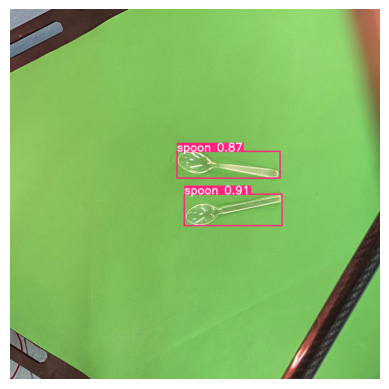
\includegraphics[width=0.21\textwidth]{figures/prob4-2.png}
  } \vfill
  \subfigure{
    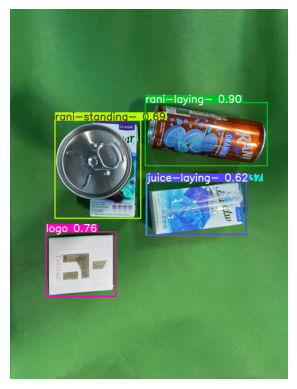
\includegraphics[width=0.21\textwidth]{figures/prob4-3.png}
  } \hfill
  \subfigure{
    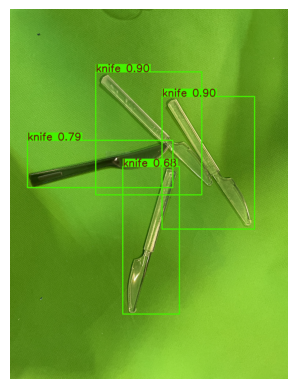
\includegraphics[width=0.21\textwidth]{figures/prob4-4.png}
  }
  \caption{Four plain examples of boundary boxes drawn with YOLO}
  \label{fig:prob4-f}
\end{figure}

\begin{figure}[htbp]
  \centering
  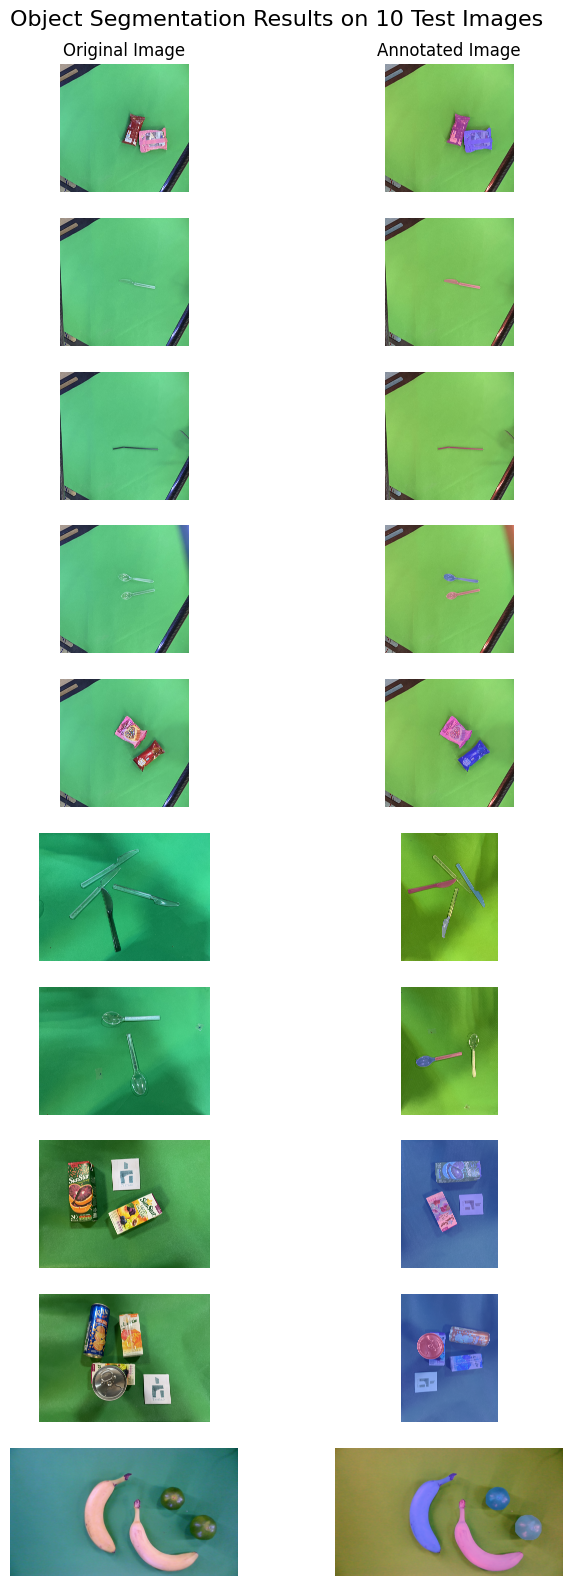
\includegraphics[width=0.48\textwidth]{figures/prob5.png}
  \caption{Object segmentation on 10 test images via FastSAM}
  \label{fig:prob5}
\end{figure}
% \vspace{10px}

\section{Conclusion}
\textbf{
  Integrating YOLO for detection and FastSAM for segmentation creates a powerful real-time visual analysis system. This combination leverages YOLO's speed and accuracy with FastSAM's precision, improving performance in tasks requiring detailed object analysis. The project demonstrates significant enhancements in accuracy and efficiency, with potential for further optimization and applications.
}

% \vspace{10px}
\begin{thebibliography}{00}
  \bibitem{b1} OpenAI. (2024). ChatGPT [Large language model]. \url{https://chatgpt.com}

  \bibitem{b2} Cong, Xiaohan; Li, Shixin; Chen, Fankai; Liu, Chen; Meng, Yue. (2023). ``A Review of YOLO Object Detection Algorithms based on Deep Learning''. Frontiers in Computing and Intelligent Systems. 4. 17-20. 10.54097/fcis.v4i2.9730.

  \bibitem{b3} Ultralytics, ``YOLO'', \url{https://docs.ultralytics.com/}

  \bibitem{b4} Glenn, Jocher, PyPi, ``ultralytics'', \url{https://pypi.org/project/ultralytics/}

  \bibitem{b5} Google Colab, ``How to segment anything with fast SAM'', \url{https://colab.research.google.com/github/roboflow-ai/notebooks/blob/main/notebooks/how-to-segment-anything-with-fast-sam.ipynb}
\end{thebibliography}
\vspace{80px}

\end{document}
